\documentclass[12pt, a4paper]{article}

% --- Packages ---
\usepackage[utf8]{inputenc}
\usepackage{mathptmx}
\usepackage[margin=1in]{geometry}
\usepackage{graphicx}
\usepackage{xcolor}
\usepackage{fancyhdr}
\usepackage{titlesec}
\usepackage{array}
\usepackage{tabularx}
\usepackage{setspace}
\usepackage{float}
\usepackage{enumitem}
\usepackage{booktabs}
\usepackage{longtable}
\usepackage{caption}
\usepackage{subcaption}
\usepackage{amsmath}
\usepackage{listings}
\usepackage[hidelinks]{hyperref}
\usepackage{tikz}
\usepackage{pgfplots}
\pgfplotsset{compat=1.18}
\usetikzlibrary{arrows.meta, positioning, shapes.geometric, calc, shapes.multipart, fit, backgrounds}

% --- Custom formatting ---
\setstretch{1.5}
\setlength{\headheight}{15pt}
\setlength{\parindent}{0pt}
\setlength{\parskip}{10pt}

% Custom colors
\definecolor{phgreen}{RGB}{169, 209, 142}
\definecolor{blockbg}{RGB}{245, 245, 245}
\definecolor{primaryblue}{RGB}{41, 128, 185}
\definecolor{secondarygreen}{RGB}{39, 174, 96}
\definecolor{warnorange}{RGB}{230, 126, 34}

% Code listing style
\lstset{
	basicstyle=\ttfamily\small,
	breaklines=true,
	frame=single,
	numbers=left,
	numberstyle=\tiny,
	tabsize=2,
	backgroundcolor=\color{blockbg}
}

% Section headings
\titleformat{\section}[block]{\normalfont\Large\bfseries\filcenter}{\thesection.}{0.5em}{}
\titleformat{\subsection}[hang]{\normalfont\large\bfseries}{\thesubsection}{0.5em}{}
\titleformat{\subsubsection}[hang]{\normalfont\normalsize\bfseries}{\thesubsubsection}{0.5em}{}

% Section spacing
\titlespacing*{\section}{0pt}{18pt plus 4pt minus 2pt}{10pt plus 2pt minus 2pt}
\titlespacing*{\subsection}{0pt}{14pt plus 3pt minus 2pt}{8pt plus 2pt minus 2pt}

% Header and Footer
\pagestyle{fancy}
\fancyhf{}
\renewcommand{\footrule}{\vspace{-5pt}\hrule height 0.5pt \vspace{1pt}\hrule height 1pt \vspace{3pt}}

\fancyhead[R]{Smart Energy Meter}
\fancyfoot[L]{\small Department of Information Technology, GHRCEM, Pune, Summer 2026}
\fancyfoot[R]{\thepage}

\begin{document}
	
	% ==========================================
	% PAGE 1: TITLE PAGE
	% ==========================================
	\thispagestyle{empty}
	\begin{center}
		\vspace*{0.5cm}
		{\Large \textbf{Mini Project Report}}\\[0.5cm]
		{\small \textbf{on}}\\[0.5cm]
		\makebox[0.8\textwidth]{\Large \textbf{Smart Energy Meter}}\\[1cm]
		
		{\small Submitted to Savitribai Phule Pune University, Pune, as a part of the academic course work\\ requirements for the completion of}\\[1cm]
		
		{\Large \textbf{Third Year Bachelor of Technology}}\\[0.3cm]
		{\small \textbf{in}}\\[0.3cm]
		{\Large \textbf{Information Technology}}\\[0.5cm]
		
		{\small Submitted by}\\[0.5cm]
		
		% Green highlighted table for students
		
		\begin{tabular}{ll}
			\textbf{Raman Bhise} & \textbf{Roll No: B52} \\
			\textbf{Panchakshari Chakor} & \textbf{Roll No: B53} \\
			\textbf{Rutika Parekar} & \textbf{Roll No: B60} \\
			\textbf{Omkar Jagtap} & \textbf{Roll No: B65} \\
		\end{tabular}
		\\[1cm]
		
		% PLACEHOLDER FOR MAIN LOGO
		% Replace 'logo_main.png' with your actual image file name
		
\includegraphics[width=0.3\textwidth]{ghrcem.png}
		
		{\large \textbf{Department of Information Technology}}\\[0.5cm]
		{\Large \textbf{G H Raisoni College of Engineering and Management, Pune}}\\[1cm]
		
		{\small Academic Year: 2025-26}\\[0.2cm]
		{\small Summer 2026}
	\end{center}
	
	\newpage
	
	% ==========================================
	% PAGE 2: CERTIFICATE
	% ==========================================
	\thispagestyle{empty}
	\begin{center}
		% PLACEHOLDER FOR NAAC LOGO
		% Replace 'logo_naac.png' with your actual image file name
		
\includegraphics[width=0.8\textwidth]{Picture2.png} %
		\vspace{0.8cm}
		
		{\Large \textbf{CERTIFICATE}}\\[1cm]
	\end{center}
	
	\begin{center}
		This is to certify that the Microproject report entitled
	\end{center}
	
	\begin{center}
		\makebox[0.8\textwidth]{\Large \textbf{Smart Energy Meter}}\\[0.5cm]
		Submitted by\\[0.5cm]
		
		\begin{tabular}{ll}
			\textbf{Raman Bhise} & \textbf{Roll No: B52} \\
			\textbf{Panchakshari Chakor} & \textbf{Roll No: B53} \\
			\textbf{Rutika Parekar} & \textbf{Roll No: B60} \\
			\textbf{Omkar Jagtap} & \textbf{Roll No: B65} \\
		\end{tabular}
		
	\end{center}
	
	\vspace{0.5cm}
	\noindent are bona fide students of this institute and have completed the coursework and Mini Project (Machine
	Learning \& IoT) (23UITELP3602) under the supervision of \textbf{Prof. Dasganu Hake}. This report is approved for partial fulfilment of the requirements of the S.Y B.Tech. (Information Technology) for the academic year 2025–26.\\[0.5cm]
	
	\noindent
	\begin{tabular*}{\textwidth}{@{\extracolsep{\fill}}lr}
		\textbf{Prof. Dasganu Hake} & \textbf{Dr. Poonam Gupta} \\
		Guide & Head of Department \\
	\end{tabular*}\\[0.5cm]
	
	\noindent
	\begin{tabular*}{\textwidth}{@{\extracolsep{\fill}}lr}
		\colorbox{phgreen}{\textbf{External Examiner Name}} & \textbf{Dr. N. B. Hulle} \\
		External Examiner & I/C Director \\
		& GHRCEM, Pune \\
	\end{tabular*}\\[0.5cm]
	
	\noindent \textbf{Date: 07/04/2026}\\
	\noindent \textbf{Place: Pune}
	
	\newpage
	
	% ==========================================
	% PAGE 3: ACKNOWLEDGMENT
	% ==========================================
	\thispagestyle{empty}
	\begin{center}
		{\Large \textbf{ACKNOWLEDGMENT}}\\[1cm]
	\end{center}
	
	\begin{spacing}{1.5}
		\noindent We would like to express our sincere thanks to \textbf{Dr. Poonam Gupta} Head of Information Technology Department, for continuous support \& valuable suggestions. We would like to thank \textbf{Prof. Dasganu Hake}, for his valuable support in providing us with the required information, guidance and light of knowledge, we could complete this Microproject.\\
		
		\noindent We take this opportunity to thank all the staff members of the Department of Information Technology Engineering for their help whenever required.\\
		
		\noindent We take this opportunity to thank our In-Charge Director, \textbf{Dr. N. B. Hulle} and Campus Director, \textbf{Dr. R. D. Kharadkar}, for his whole hearted support, motivation \& valuable suggestions.\\
		
		\noindent Finally, we would like to give special thanks to all staff members of the \textbf{Department of Information Technology}, G H Raisoni College of Engineering and Management, Pune \& our friends for their kind support.\\[0.5cm]
	\end{spacing}

	
	\begin{tabular}{ll}
		Raman Bhise & (B Roll no. 52) \\
		Panchakshari Chakor & (B Roll no. 53) \\
		Rutika Parekar & (B Roll no. 60) \\
		Omkar Jagtap & (B Roll no. 65) \\
	\end{tabular}
	
	
	\newpage
	
	% ==========================================
	% PAGE 4: ABSTRACT
	% ==========================================
	\thispagestyle{empty}
	\begin{center}
		{\Large \textbf{ABSTRACT}}\\[1cm]
	\end{center}
	
	This project is a per-appliance energy monitoring system. Most electricity bills show a single monthly figure for the entire household. There is no way to know which device consumes the most power or whether an appliance has developed a fault that causes it to draw excess current.
	
	We built a monitoring unit using an ESP32 DevKit V1 microcontroller. The device connects between a wall socket and an appliance, measuring voltage with a ZMPT101B transformer sensor and current with an ACS712 20A Hall-effect sensor. The firmware samples both waveforms at 200 points per cycle and computes RMS voltage, RMS current, real power, and cumulative energy in kWh.
	
	Telemetry data transmits to a Flask backend server over WiFi using the MQTT protocol. The backend runs three machine learning models: a LightGBM regressor for power prediction, a binary classifier for on/off state detection, and an Isolation Forest for anomaly detection. When a reading deviates from the expected baseline, the dashboard displays an alert.
	
	The hardware includes a 128x64 OLED display for local readings and a 5V relay module for remote control. Users can toggle appliances from a web dashboard, which shows live readings, historical charts, and estimated costs.
	
	We tested the system on an electric kettle (600W) and a laptop charger (65W). Measurements matched a commercial power meter within 2\% after calibration. The total component cost is approximately Rs. 1,500 per unit.
	
	\newpage
	
	% ==========================================
	% PAGE 5: INDEX
	% ==========================================
	\thispagestyle{empty}
	\begin{center}
		{\Large \textbf{Index}}\\[1cm]
	\end{center}
	
	\renewcommand{\arraystretch}{2} % Taller rows to match the document
	\begin{center}
		\begin{tabular}{|c|p{0.6\textwidth}|c|}
			\hline
			\textbf{S N} & \textbf{Details} & \textbf{Page No.} \\ \hline
			\textbf{1} & \textbf{Introduction} & 1 \\ \hline
			\textbf{2} & \textbf{Objective of the Project} & 5 \\ \hline
			\textbf{3} & \textbf{Hardware and Software} & 7 \\ \hline
			\textbf{4} & \textbf{Project Design / Methodology} & 12 \\ \hline
			\textbf{5} & \textbf{Implementation / Working} & 17 \\ \hline
			\textbf{6} & \textbf{Results / Output} & 21 \\ \hline
			\textbf{7} & \textbf{Conclusion} & 27 \\ \hline
			\textbf{8} & \textbf{References} & 29 \\ \hline
		\end{tabular}
	\end{center}
	\renewcommand{\arraystretch}{1} % Reset array stretch for rest of doc
	
	
	\newpage
	
	% ==========================================
	% PAGE 6: INTRODUCTION (Header/Footer start)
	% ==========================================
	% Enable the fancy style and start counting pages at 1
	\pagestyle{fancy}
	\setcounter{page}{1}
	
	\section{INTRODUCTION}
	
	\subsection{Overview}
	
	This project is a per-appliance energy monitoring system built around the ESP32 DevKit V1 microcontroller. The device connects between a wall socket and an appliance to measure voltage, current, and power in real time. Figure~\ref{fig:system-overview} shows the high-level system architecture.
	
	\begin{figure}[H]
		\centering
		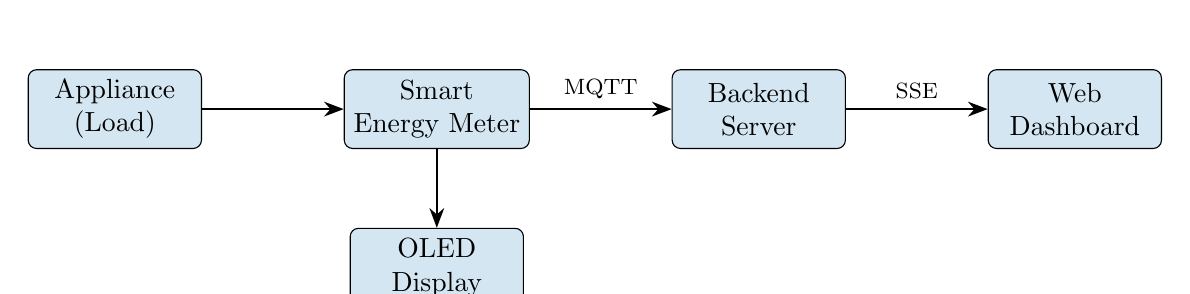
\begin{tikzpicture}[
			node distance=1.8cm,
			block/.style={rectangle, draw, fill=primaryblue!20, minimum width=2.2cm, minimum height=1cm, align=center, rounded corners=3pt},
			arrow/.style={-{Stealth[length=2.5mm]}, thick}
		]
		\node[block] (appliance) {Appliance\\(Load)};
		\node[block, right=of appliance] (meter) {Smart\\Energy Meter};
		\node[block, right=of meter] (cloud) {Backend\\Server};
		\node[block, right=of cloud] (dashboard) {Web\\Dashboard};
		\node[block, below=1cm of meter] (oled) {OLED\\Display};
		
		\draw[arrow] (appliance) -- (meter);
		\draw[arrow] (meter) -- node[above, font=\footnotesize] {MQTT} (cloud);
		\draw[arrow] (cloud) -- node[above, font=\footnotesize] {SSE} (dashboard);
		\draw[arrow] (meter) -- (oled);
		\end{tikzpicture}
		\caption{High-level system architecture}
		\label{fig:system-overview}
	\end{figure}
	
	The hardware consists of the following components:
	
	\begin{itemize}[itemsep=2pt, topsep=6pt]
		\item \textbf{ZMPT101B AC voltage sensor:} Measures mains voltage in the range of 0--250V AC. The sensor uses a miniature transformer to step down the voltage and provide galvanic isolation.
		
		\item \textbf{ACS712 20A current sensor:} Measures load current using the Hall effect. The sensor outputs a voltage proportional to the current flowing through it, with 100mV per ampere sensitivity.
		
		\item \textbf{HLK-PM01 power supply:} Converts 230V AC mains to 5V DC with isolation. This module powers the entire circuit safely.
		
		\item \textbf{ESP32 DevKit V1:} The main microcontroller with dual-core 240MHz processor, built-in WiFi, and 12-bit ADC. It handles all computation and communication.
		
		\item \textbf{SSD1306 OLED display:} A 128$\times$64 pixel monochrome display that shows voltage, current, power, and energy readings locally.
		
		\item \textbf{5V relay module:} Allows remote on/off control of the connected appliance through the web dashboard.
		
		\item \textbf{TTP223 touch sensor:} Provides a capacitive touch interface for manual relay control and display navigation.
	\end{itemize}
	
	The firmware samples voltage and current waveforms at 200 points per measurement cycle (20ms at 50Hz). It computes RMS values and transmits data to a backend server using the MQTT protocol. The server stores readings and runs machine learning models to detect unusual consumption patterns. Users access a web dashboard that shows live readings, historical charts, and relay controls.
	
	The main difference between this system and whole-house smart meters is granularity. Each monitoring unit connects to one appliance and reports its consumption separately. This approach provides three advantages:
	
	\begin{enumerate}[itemsep=3pt, topsep=6pt]
		\item Identification of which specific device is consuming power
		\item Detection of faults at the individual device level
		\item Targeted control of individual loads through the relay
	\end{enumerate}
	
	\newpage
	
	\subsection{Motivation}
	
	Most smart meters installed in homes measure total energy consumption for an entire premises. A household running an air conditioner, water heater, and refrigerator simultaneously sees only one combined kWh figure on the electricity bill. There is no way to determine which appliance caused a spike in consumption, or whether a particular device has developed a fault and is drawing more power than expected.
	
	Figure~\ref{fig:problem} illustrates this problem. Traditional meters provide only the total consumption, while our system provides individual appliance data.
	
	\begin{figure}[H]
		\centering
		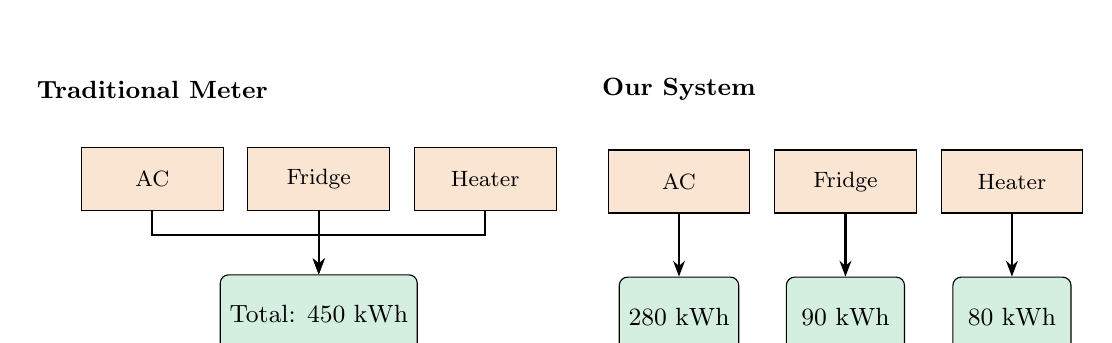
\begin{tikzpicture}[
			node distance=0.8cm,
			appliance/.style={rectangle, draw, fill=warnorange!20, minimum width=1.8cm, minimum height=0.8cm, align=center, font=\footnotesize},
			meter/.style={rectangle, draw, fill=secondarygreen!20, minimum width=2cm, minimum height=1cm, align=center, font=\small, rounded corners=3pt},
			arrow/.style={-{Stealth[length=2mm]}, thick}
		]
		% Traditional side
		\node[font=\small\bfseries] (trad-label) {Traditional Meter};
		\node[appliance, below=0.5cm of trad-label] (ac) {AC};
		\node[appliance, right=0.3cm of ac] (fridge) {Fridge};
		\node[appliance, right=0.3cm of fridge] (heater) {Heater};
		\node[meter, below=0.8cm of fridge] (trad-meter) {Total: 450 kWh};
		
		\draw[arrow] (ac.south) -- ++(0,-0.3) -| (trad-meter.north);
		\draw[arrow] (fridge) -- (trad-meter);
		\draw[arrow] (heater.south) -- ++(0,-0.3) -| (trad-meter.north);
		
		% Our system side
		\node[font=\small\bfseries, right=4cm of trad-label] (our-label) {Our System};
		\node[appliance, below=0.5cm of our-label] (ac2) {AC};
		\node[appliance, right=0.3cm of ac2] (fridge2) {Fridge};
		\node[appliance, right=0.3cm of fridge2] (heater2) {Heater};
		\node[meter, below=0.8cm of ac2, minimum width=1.5cm] (m1) {280 kWh};
		\node[meter, below=0.8cm of fridge2, minimum width=1.5cm] (m2) {90 kWh};
		\node[meter, below=0.8cm of heater2, minimum width=1.5cm] (m3) {80 kWh};
		
		\draw[arrow] (ac2) -- (m1);
		\draw[arrow] (fridge2) -- (m2);
		\draw[arrow] (heater2) -- (m3);
		\end{tikzpicture}
		\caption{Comparison: Traditional metering vs. per-appliance metering}
		\label{fig:problem}
	\end{figure}
	
	The lack of device-level visibility creates the following problems:
	
	\begin{itemize}[itemsep=2pt, topsep=4pt]
		\item \textbf{No consumption breakdown:} Users cannot identify which appliances consume the most electricity or contribute most to the bill.
		
		\item \textbf{Hidden faults:} Faulty equipment drawing excess power may go unnoticed until complete failure, potentially causing higher bills or safety hazards.
		
		\item \textbf{No feedback loop:} Energy conservation efforts lack measurable feedback. Users cannot verify if turning off standby devices actually reduces their bill.
		
		\item \textbf{No remote control:} Individual devices cannot be controlled remotely, which limits automation possibilities.
	\end{itemize}
	
	Non-Intrusive Load Monitoring (NILM) systems attempt to disaggregate total consumption into per-device estimates using signal processing algorithms. However, NILM requires expensive high-frequency sensors at the main distribution board, and the results are probabilistic rather than exact.
	
	The ESP32 DevKit V1 costs approximately Rs. 450 and includes WiFi connectivity. Combined with inexpensive sensor modules (Rs. 150--200 each), it becomes feasible to deploy one monitoring unit per appliance instead of relying on estimation algorithms.
	
	\subsection{Scope and Limitation}
	
	The system targets single-phase residential and small commercial installations operating on 230V AC, 50Hz supply. Table~\ref{tab:specs} lists the system specifications.
	
	\begin{table}[H]
		\centering
		\caption{System specifications}
		\label{tab:specs}
		\vspace{6pt}
		\begin{tabular}{|l|l|}
			\hline
			\textbf{Parameter} & \textbf{Specification} \\
			\hline
			Input voltage range & 100--250V AC \\
			Frequency & 50/60 Hz \\
			Maximum current & 20A \\
			Measurement accuracy & $\pm$2\% (after calibration) \\
			Communication & WiFi 802.11 b/g/n (2.4 GHz) \\
			Protocol & MQTT over TCP \\
			Relay rating & 10A at 250V AC (resistive) \\
			\hline
		\end{tabular}
	\end{table}
	
	\textbf{Limitations:}
	
	\begin{itemize}[itemsep=2pt, topsep=6pt]
		\item \textbf{Single-phase only:} Three-phase industrial installations are not supported by this version.
		
		\item \textbf{Current limit:} The ACS712-20A sensor saturates above 20A. High-power appliances like geysers (above 4kW) need a different sensor variant.
		
		\item \textbf{WiFi dependency:} Backend features (dashboard, ML alerts) require network connectivity. Local display works offline.
		
		\item \textbf{Relay rating:} The relay handles 10A resistive loads safely. Inductive loads like motors may require additional snubber circuits.
		
		\item \textbf{Model drift:} ML predictions may become less accurate over time if usage patterns change significantly.
	\end{itemize}
	
	\newpage
	
	% ==========================================
	% PAGE 7: OBJECTIVE
	% ==========================================
	\section{Objective of the Project}
	
	\subsection{Problem Statement}
	
	Electricity bills show a single monthly kWh figure for the entire household. This aggregate measurement does not answer practical questions that users commonly have:
	
	\begin{itemize}[itemsep=1pt, topsep=1pt]
		\item Which appliance uses the most power?
		\item Has a device started drawing more current than usual?
		\item Can I turn off a specific appliance remotely?
		\item Is a particular device faulty and wasting electricity?
	\end{itemize}
	
	Whole-house smart meters do not break down consumption by device. Non-Intrusive Load Monitoring (NILM) systems attempt to estimate per-device loads from the total household signal, but they require high-resolution current sensing at the distribution board, and the readings are probabilistic rather than exact.
	
	Without device-level metering, users cannot identify appliances that are over-consuming due to faults, cannot measure whether behavior changes reduce consumption, and cannot control devices remotely.
	
	\subsection{Proposed Solution}
	
	The system is a single-appliance monitoring module that connects between the wall outlet and the appliance. Each unit measures the exact electrical parameters of its connected device, removing the ambiguity of aggregate metering. Figure~\ref{fig:layers} shows the four-layer architecture.
	
	\begin{figure}[H]
		\centering
		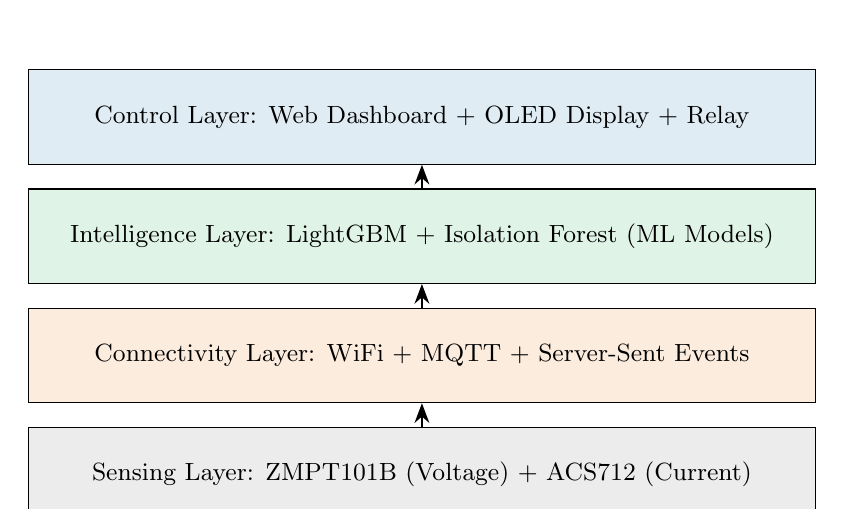
\begin{tikzpicture}[
			layer/.style={rectangle, draw, minimum width=10cm, minimum height=1.2cm, align=center, font=\small},
			arrow/.style={-{Stealth[length=2.5mm]}, thick}
		]
		\node[layer, fill=primaryblue!15] (control) {Control Layer: Web Dashboard + OLED Display + Relay};
		\node[layer, fill=secondarygreen!15, below=0.3cm of control] (intel) {Intelligence Layer: LightGBM + Isolation Forest (ML Models)};
		\node[layer, fill=warnorange!15, below=0.3cm of intel] (conn) {Connectivity Layer: WiFi + MQTT + Server-Sent Events};
		\node[layer, fill=gray!15, below=0.3cm of conn] (sense) {Sensing Layer: ZMPT101B (Voltage) + ACS712 (Current)};
		
		\draw[arrow] (sense) -- (conn);
		\draw[arrow] (conn) -- (intel);
		\draw[arrow] (intel) -- (control);
		\end{tikzpicture}
		\caption{Four-layer system architecture}
		\label{fig:layers}
	\end{figure}

	\begin{itemize}[itemsep=3pt, topsep=4pt]
		\item \textbf{Sensing layer:} The ZMPT101B voltage transformer samples the AC supply waveform in parallel. The ACS712 20A current sensor measures load current in series. The ESP32's 12-bit ADC digitizes both signals at 200 samples per measurement cycle (20ms window). From these samples, the firmware computes:
		\begin{itemize}[itemsep=2pt, topsep=4pt]
			\item RMS voltage and RMS current
			\item Real power and apparent power
			\item Power factor
			\item Cumulative energy consumption (kWh)
		\end{itemize}
		
		\item \textbf{Connectivity layer:} The ESP32 connects to the local WiFi network and maintains a persistent MQTT connection with the backend broker. Telemetry publishes at configurable intervals (default: 5 seconds). For events that require instant notification (anomaly alerts, relay state changes), Server-Sent Events push updates to connected dashboards.
		
		\item \textbf{Intelligence layer:} The backend runs three ML models trained on historical energy data:
		\begin{itemize}[itemsep=2pt, topsep=4pt]
			\item LightGBM regressor for power prediction
			\item LightGBM binary classifier for on/off state detection
			\item Isolation Forest for anomaly detection
		\end{itemize}
		
		\item \textbf{Control layer:} The web dashboard displays live consumption, historical charts, and cost estimates. A relay on the hardware allows remote switching. The local OLED display shows readings when network connectivity is unavailable.
	\end{itemize}
	
	\newpage
	
	% ==========================================
	% PAGE 8: TOOLS/TECHNOLOGIES
	% ==========================================
	\section{Tools and Technologies Used}
	
	\subsection{Hardware Specifications}
	
	The system uses the following IoT modules and sensors. Table~\ref{tab:hardware} provides detailed specifications.
	
	\begin{table}[H]
		\centering
		\caption{Hardware modules and specifications}
		\label{tab:hardware}
		\vspace{6pt}
		\begin{tabular}{|l|l|p{6.5cm}|}
			\hline
			\textbf{Module} & \textbf{Model} & \textbf{Function} \\
			\hline
			Microcontroller & ESP32 DevKit V1 & Dual-core 240MHz processor with WiFi 802.11 b/g/n. Two 12-bit ADCs for analog sensing. 520KB SRAM, 4MB flash. Built-in USB-UART and 3.3V regulator. \\
			\hline
			Voltage sensor & ZMPT101B & Miniature voltage transformer. Input 0--250V AC, output 0--3.3V centered at VCC/2. Provides 4kV isolation. \\
			\hline
			Current sensor & ACS712-20A & Hall-effect sensor with 100mV/A sensitivity. Zero-current output at VCC/2. Isolation 2.1kV RMS. \\
			\hline
			Display & SSD1306 128$\times$64 & Monochrome OLED with I2C interface. Shows local readings without network. \\
			\hline
			Relay & 5V single-channel & Optocoupler-isolated, active LOW trigger. Rated 10A/250VAC resistive. \\
			\hline
			Touch sensor & TTP223 & Capacitive touch module for manual user input. \\
			\hline
			Power supply & HLK-PM01 & AC-DC isolated converter, 230V AC input to 5V/0.6A DC output. \\
			\hline
		\end{tabular}
	\end{table}
	
	\begin{table}[H]
		\centering
		\caption{Bill of materials with cost breakdown}
		\label{tab:bom}
		\vspace{6pt}
		\begin{tabular}{|l|r|}
			\hline
			\textbf{Component} & \textbf{Cost (INR)} \\
			\hline
			ESP32 DevKit V1 & 450 \\
			ZMPT101B & 180 \\
			ACS712-20A & 120 \\
			SSD1306 OLED 128$\times$64 & 200 \\
			5V relay module & 80 \\
			HLK-PM01 & 250 \\
			Miscellaneous (wires, enclosure, terminals) & 220 \\
			\hline
			\textbf{Total} & \textbf{1,500} \\
			\hline
		\end{tabular}
	\end{table}
	
	\subsection{Software Specifications}
	
	The software stack consists of firmware running on the ESP32 and a backend server application. Figure~\ref{fig:software-stack} shows the relationship between components.
	
	\begin{figure}[H]
		\centering
		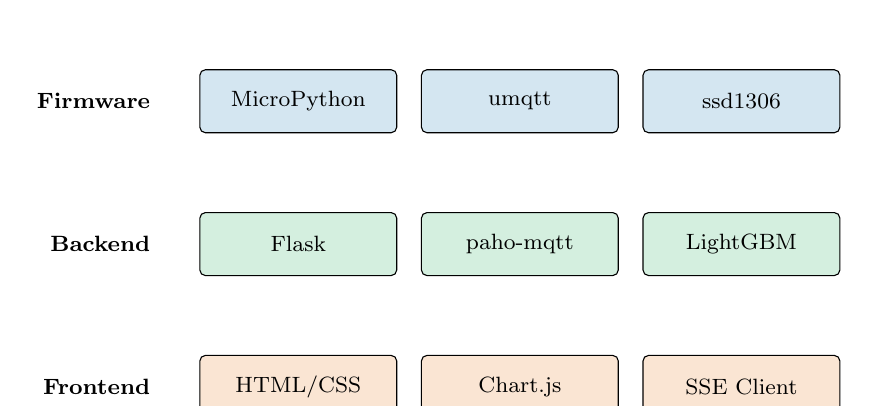
\begin{tikzpicture}[
			node distance=0.5cm,
			component/.style={rectangle, draw, minimum width=2.5cm, minimum height=0.8cm, align=center, font=\footnotesize, rounded corners=2pt},
			layer/.style={rectangle, draw, dashed, minimum width=8cm, minimum height=1.5cm, align=center}
		]
		% Firmware layer
		\node[component, fill=primaryblue!20] (mp) {MicroPython};
		\node[component, fill=primaryblue!20, right=0.3cm of mp] (mqtt-fw) {umqtt};
		\node[component, fill=primaryblue!20, right=0.3cm of mqtt-fw] (ssd) {ssd1306};
		
		% Backend layer
		\node[component, fill=secondarygreen!20, below=1cm of mp] (flask) {Flask};
		\node[component, fill=secondarygreen!20, right=0.3cm of flask] (paho) {paho-mqtt};
		\node[component, fill=secondarygreen!20, right=0.3cm of paho] (lgbm) {LightGBM};
		
		% Frontend layer
		\node[component, fill=warnorange!20, below=1cm of flask] (html) {HTML/CSS};
		\node[component, fill=warnorange!20, right=0.3cm of html] (chartjs) {Chart.js};
		\node[component, fill=warnorange!20, right=0.3cm of chartjs] (sse) {SSE Client};
		
		% Labels
		\node[left=0.5cm of mp, font=\footnotesize\bfseries] {Firmware};
		\node[left=0.5cm of flask, font=\footnotesize\bfseries] {Backend};
		\node[left=0.5cm of html, font=\footnotesize\bfseries] {Frontend};
		\end{tikzpicture}
		\caption{Software stack components}
		\label{fig:software-stack}
	\end{figure}
	
	\textbf{Firmware:} The firmware runs MicroPython 1.23 on the ESP32 DevKit V1. We chose MicroPython over C/Arduino for the following reasons:
	
	\begin{itemize}[itemsep=3pt, topsep=4pt]
		\item Faster prototyping with Python syntax
		\item Interactive REPL for debugging
		\item Built-in libraries for MQTT and I2C
		\item Easier modification without recompilation
	\end{itemize}
	
	\textbf{Backend:} The server runs Python 3.11 with Flask for HTTP endpoints. The paho-mqtt library handles MQTT subscriptions. NanoMQ serves as a lightweight MQTT broker that runs on low-resource servers.
	
	\textbf{Frontend:} The web dashboard uses HTML, CSS, and JavaScript. Chart.js renders the historical power graph. Server-Sent Events (SSE) push live data to the browser without polling.
	
	\begin{table}[H]
		\centering
		\caption{Software stack summary}
		\label{tab:software}
		\vspace{6pt}
		\begin{tabular}{|l|l|l|}
			\hline
			\textbf{Layer} & \textbf{Technology} & \textbf{Purpose} \\
			\hline
			Firmware & MicroPython 1.23 & Sensor reading, RMS calculation, MQTT \\
			Backend framework & Flask 3.0 & HTTP API, SSE streaming \\
			MQTT client & paho-mqtt & Subscribe to telemetry topics \\
			MQTT broker & NanoMQ & Message routing between devices \\
			ML libraries & LightGBM, scikit-learn & Prediction and anomaly detection \\
			Frontend charts & Chart.js 4.4 & Historical power visualization \\
			\hline
		\end{tabular}
	\end{table}
	
	\subsection{Machine Learning Algorithm}
	
	The backend runs three machine learning models to analyze energy consumption patterns. Figure~\ref{fig:ml-pipeline} shows how data flows through the ML pipeline.
	
	\begin{figure}[H]
		\centering
		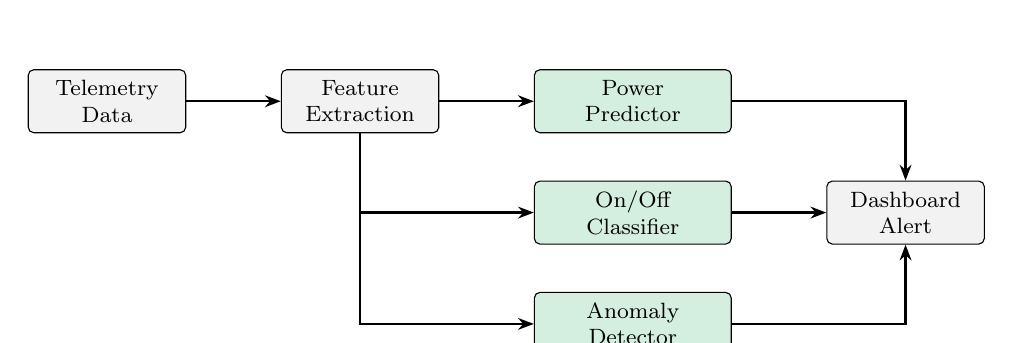
\begin{tikzpicture}[
			node distance=1.2cm,
			block/.style={rectangle, draw, fill=gray!10, minimum width=2cm, minimum height=0.8cm, align=center, font=\footnotesize, rounded corners=2pt},
			model/.style={rectangle, draw, fill=secondarygreen!20, minimum width=2.5cm, minimum height=0.8cm, align=center, font=\footnotesize, rounded corners=2pt},
			arrow/.style={-{Stealth[length=2mm]}, thick}
		]
		\node[block] (input) {Telemetry\\Data};
		\node[block, right=of input] (features) {Feature\\Extraction};
		\node[model, right=of features] (predictor) {Power\\Predictor};
		\node[model, below=0.6cm of predictor] (classifier) {On/Off\\Classifier};
		\node[model, below=0.6cm of classifier] (anomaly) {Anomaly\\Detector};
		\node[block, right=of classifier] (output) {Dashboard\\Alert};
		
		\draw[arrow] (input) -- (features);
		\draw[arrow] (features) -- (predictor);
		\draw[arrow] (features) |- (classifier);
		\draw[arrow] (features) |- (anomaly);
		\draw[arrow] (predictor) -| (output);
		\draw[arrow] (classifier) -- (output);
		\draw[arrow] (anomaly) -| (output);
		\end{tikzpicture}
		\caption{ML pipeline data flow}
		\label{fig:ml-pipeline}
	\end{figure}
	
	\newpage
	\textbf{Power predictor (LightGBM regression):} This model predicts expected power consumption based on:
	
	\begin{itemize}[itemsep=2pt, topsep=4pt]
		\item Time features: hour of day, day of week, month, season
		\item Lag features: consumption in the last 1, 6, and 24 hours
		\item Rolling statistics: 6-hour and 24-hour moving averages
	\end{itemize}
	
	LightGBM (Light Gradient Boosting Machine) is a gradient boosting framework that builds an ensemble of decision trees. It performs well on tabular data with temporal patterns.
	
	\textbf{On/off classifier (LightGBM binary classification):} This model predicts whether an appliance should be on or off at a given time. It uses the same feature set as the power predictor. The training data has class imbalance (appliances are off more often than on), so we apply class weights during training to compensate.
	
	\textbf{Anomaly detector (Isolation Forest with Z-score):} This detector flags readings that deviate from normal operation. Two methods work together:
	
	\begin{itemize}[leftmargin=*, itemsep=2pt, topsep=4pt]
		\item Isolation Forest detects structural anomalies by building random trees and measuring how quickly each sample gets isolated
		\item Z-score detects simple spikes by measuring standard deviations from the mean
	\end{itemize}
	
	A reading is flagged if either method triggers. The contamination parameter is set to 2\%, meaning the model expects roughly 2\% of readings to be anomalous.
	
	\textbf{Training data:} The models train on hourly aggregated data from the AMPds (Almanac of Minutely Power dataset), a public dataset of whole-home and individual appliance power measurements.
	
	\begin{table}[H]
		\centering
		\caption{ML model performance metrics}
		\label{tab:ml-metrics}
		\vspace{6pt}
		\begin{tabular}{|l|l|r|}
			\hline
			\textbf{Model} & \textbf{Metric} & \textbf{Value} \\
			\hline
			Power predictor & R\textsuperscript{2} score & 0.87 \\
			\hline
			On/off classifier & Accuracy & 94\% \\
			\hline
			Anomaly detector & Precision & 89\% \\
			\hline
		\end{tabular}
	\end{table}
	
	\subsection{Cloud Platform}
	
	The system deploys to a DigitalOcean droplet running Ubuntu 22.04. A \$6/month droplet (1 vCPU, 1GB RAM) handles all server components:
	
	\begin{itemize}[itemsep=2pt, topsep=4pt]
		\item NanoMQ MQTT broker for device communication
		\item Flask backend for API endpoints and ML inference
		\item Static file serving for the web dashboard
	\end{itemize}
	
	The deployment uses a simple setup without reverse proxy or SSL encryption for the development phase. Flask runs directly on port 5000. The deployment script (\texttt{deploy.sh}) automates dependency installation and service configuration.
	
	\subsection{Development Tools}
	
	The following tools were used during development:
	
	\begin{itemize}[itemsep=2pt, topsep=6pt]
		\item \textbf{VS Code} with Python and MicroPython extensions for code editing
		\item \textbf{ampy} for uploading files to ESP32 flash memory over serial
		\item \textbf{esptool.py} for flashing the MicroPython firmware binary
		\item \textbf{Git and GitHub} for version control and collaboration
		\item \textbf{MQTT Explorer} for debugging MQTT message flow
		\item \textbf{Jupyter Notebook} for ML model training and experimentation
	\end{itemize}
	
	\subsection{GitHub Link}
	
	The complete source code is available at:
	
	\url{https://github.com/lostfleetdev/Smart-Energy-Meter-IOT}
	
	\newpage
	
	\section{Project Design / Methodology}
	
	\subsection{System Architecture}
	
	The system follows a three-tier IoT architecture: edge device, backend server, and web frontend. Figure~\ref{fig:architecture} shows how data flows between the tiers.
	
	\begin{figure}[H]
		\centering
		\resizebox{0.95\textwidth}{!}{%
		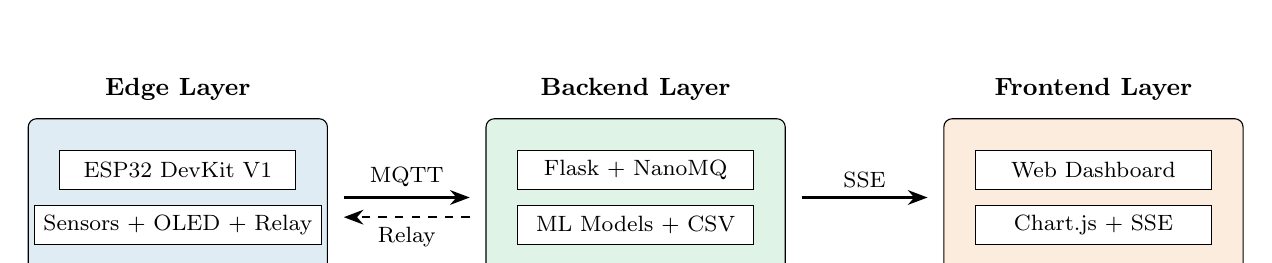
\begin{tikzpicture}[
			node distance=1.2cm,
			tier/.style={rectangle, draw, minimum width=3.8cm, minimum height=2cm, align=center, rounded corners=3pt},
			component/.style={rectangle, draw, fill=white, minimum width=3cm, minimum height=0.5cm, align=center, font=\footnotesize},
			arrow/.style={-{Stealth[length=2.5mm]}, thick},
			label/.style={font=\small\bfseries}
		]
		% Edge tier
		\node[tier, fill=primaryblue!15] (edge) {};
		\node[label, above=0.1cm of edge.north] {Edge Layer};
		\node[component, fill=white] at ([yshift=0.35cm]edge.center) {ESP32 DevKit V1};
		\node[component, fill=white] at ([yshift=-0.35cm]edge.center) {Sensors + OLED + Relay};
		
		% Backend tier
		\node[tier, fill=secondarygreen!15, right=2cm of edge] (backend) {};
		\node[label, above=0.1cm of backend.north] {Backend Layer};
		\node[component, fill=white] at ([yshift=0.35cm]backend.center) {Flask + NanoMQ};
		\node[component, fill=white] at ([yshift=-0.35cm]backend.center) {ML Models + CSV};
		
		% Frontend tier
		\node[tier, fill=warnorange!15, right=2cm of backend] (frontend) {};
		\node[label, above=0.1cm of frontend.north] {Frontend Layer};
		\node[component, fill=white] at ([yshift=0.35cm]frontend.center) {Web Dashboard};
		\node[component, fill=white] at ([yshift=-0.35cm]frontend.center) {Chart.js + SSE};
		
		% Arrows
		\draw[arrow] ([xshift=0.2cm]edge.east) -- node[above, font=\footnotesize] {MQTT} ([xshift=-0.2cm]backend.west);
		\draw[arrow] ([xshift=0.2cm]backend.east) -- node[above, font=\footnotesize] {SSE} ([xshift=-0.2cm]frontend.west);
		\draw[arrow, dashed] ([yshift=-0.25cm, xshift=-0.2cm]backend.west) -- node[below, font=\footnotesize] {Relay} ([yshift=-0.25cm, xshift=0.2cm]edge.east);
		\end{tikzpicture}%
		}
		\caption{Three-tier system architecture}
		\label{fig:architecture}
	\end{figure}
	
	\textbf{Edge layer (ESP32 DevKit V1):} The microcontroller performs several functions:
	
	\begin{itemize}[itemsep=2pt, topsep=4pt]
		\item Samples voltage and current at 200 points per measurement cycle (20ms)
		\item Computes RMS values and power factor from the raw samples
		\item Publishes JSON telemetry over MQTT at configurable intervals
		\item Displays readings on the local OLED screen
		\item Handles touch button input for local relay control
	\end{itemize}
	
	\textbf{Backend layer (Flask + NanoMQ):} The server components work together:
	
	\begin{itemize}[itemsep=2pt, topsep=4pt]
		\item NanoMQ broker accepts MQTT connections from devices
		\item Flask server subscribes to telemetry topics
		\item ML service runs inference on each incoming reading
		\item Data stores in CSV format for historical analysis
		\item Server-Sent Events push updates to connected dashboards
	\end{itemize}
	
	\textbf{Frontend layer (Web dashboard):} A single-page application that:
	
	\begin{itemize}[itemsep=2pt, topsep=4pt]
		\item Displays live readings with animated gauges
		\item Shows historical power consumption charts
		\item Provides relay on/off controls
		\item Receives real-time updates via SSE (no polling required)
	\end{itemize}
	
	\subsection{Modules of the System}
	
	The system consists of five functional modules. Each module handles a specific responsibility.
	
	\begin{itemize}[itemsep=6pt, topsep=6pt]
		\item \textbf{Sensing module:} The ZMPT101B and ACS712 sensors connect to ESP32 ADC pins. Raw ADC values pass through calibration constants to produce voltage and current readings. The sensors provide galvanic isolation between the AC mains and the low-voltage electronics.
		
		\item \textbf{Processing module:} The RMS calculation firmware samples 200 points over 20ms (one complete AC cycle at 50Hz). For each measurement cycle:
		\begin{enumerate}[itemsep=1pt, topsep=2pt]
			\item Sample ADC values in a tight loop
			\item Compute sum of squares for voltage and current
			\item Calculate RMS values: $V_{RMS} = \sqrt{\frac{1}{N}\sum v_i^2}$
			\item Calculate power factor from phase difference
			\item Accumulate energy by integrating power over time
		\end{enumerate}
		
		\item \textbf{Communication module:} ESP32 WiFi connects to the local network. The MQTT client uses two topics:
		\begin{itemize}[itemsep=1pt, topsep=2pt]
			\item Publish: \texttt{energy/\{device\_id\}/telemetry} (sensor readings)
			\item Subscribe: \texttt{energy/\{device\_id\}/relay/set} (control commands)
		\end{itemize}
		
		\item \textbf{Intelligence module:} ML models on the backend predict expected power, classify on/off state, and flag anomalies. The service loads trained models (.pkl files) at startup and runs inference on each incoming reading.

		\newpage
		\item \textbf{Interface module:} Two interfaces provide user interaction:
		\begin{itemize}[itemsep=1pt, topsep=2pt]
			\item \textbf{Local (OLED):} Four screens cycled by long-press: live readings, energy totals, relay control, debug info
			\item \textbf{Remote (Web):} Dashboard with gauges, charts, and relay toggle buttons
		\end{itemize}
	\end{itemize}
	
	\subsection{Circuit Diagram}
	
	Figure~\ref{fig:circuit} shows the complete circuit diagram of the Smart Energy Meter. The connections are described in Table~\ref{tab:gpio}.
	
	\begin{figure}[H]
		\centering
		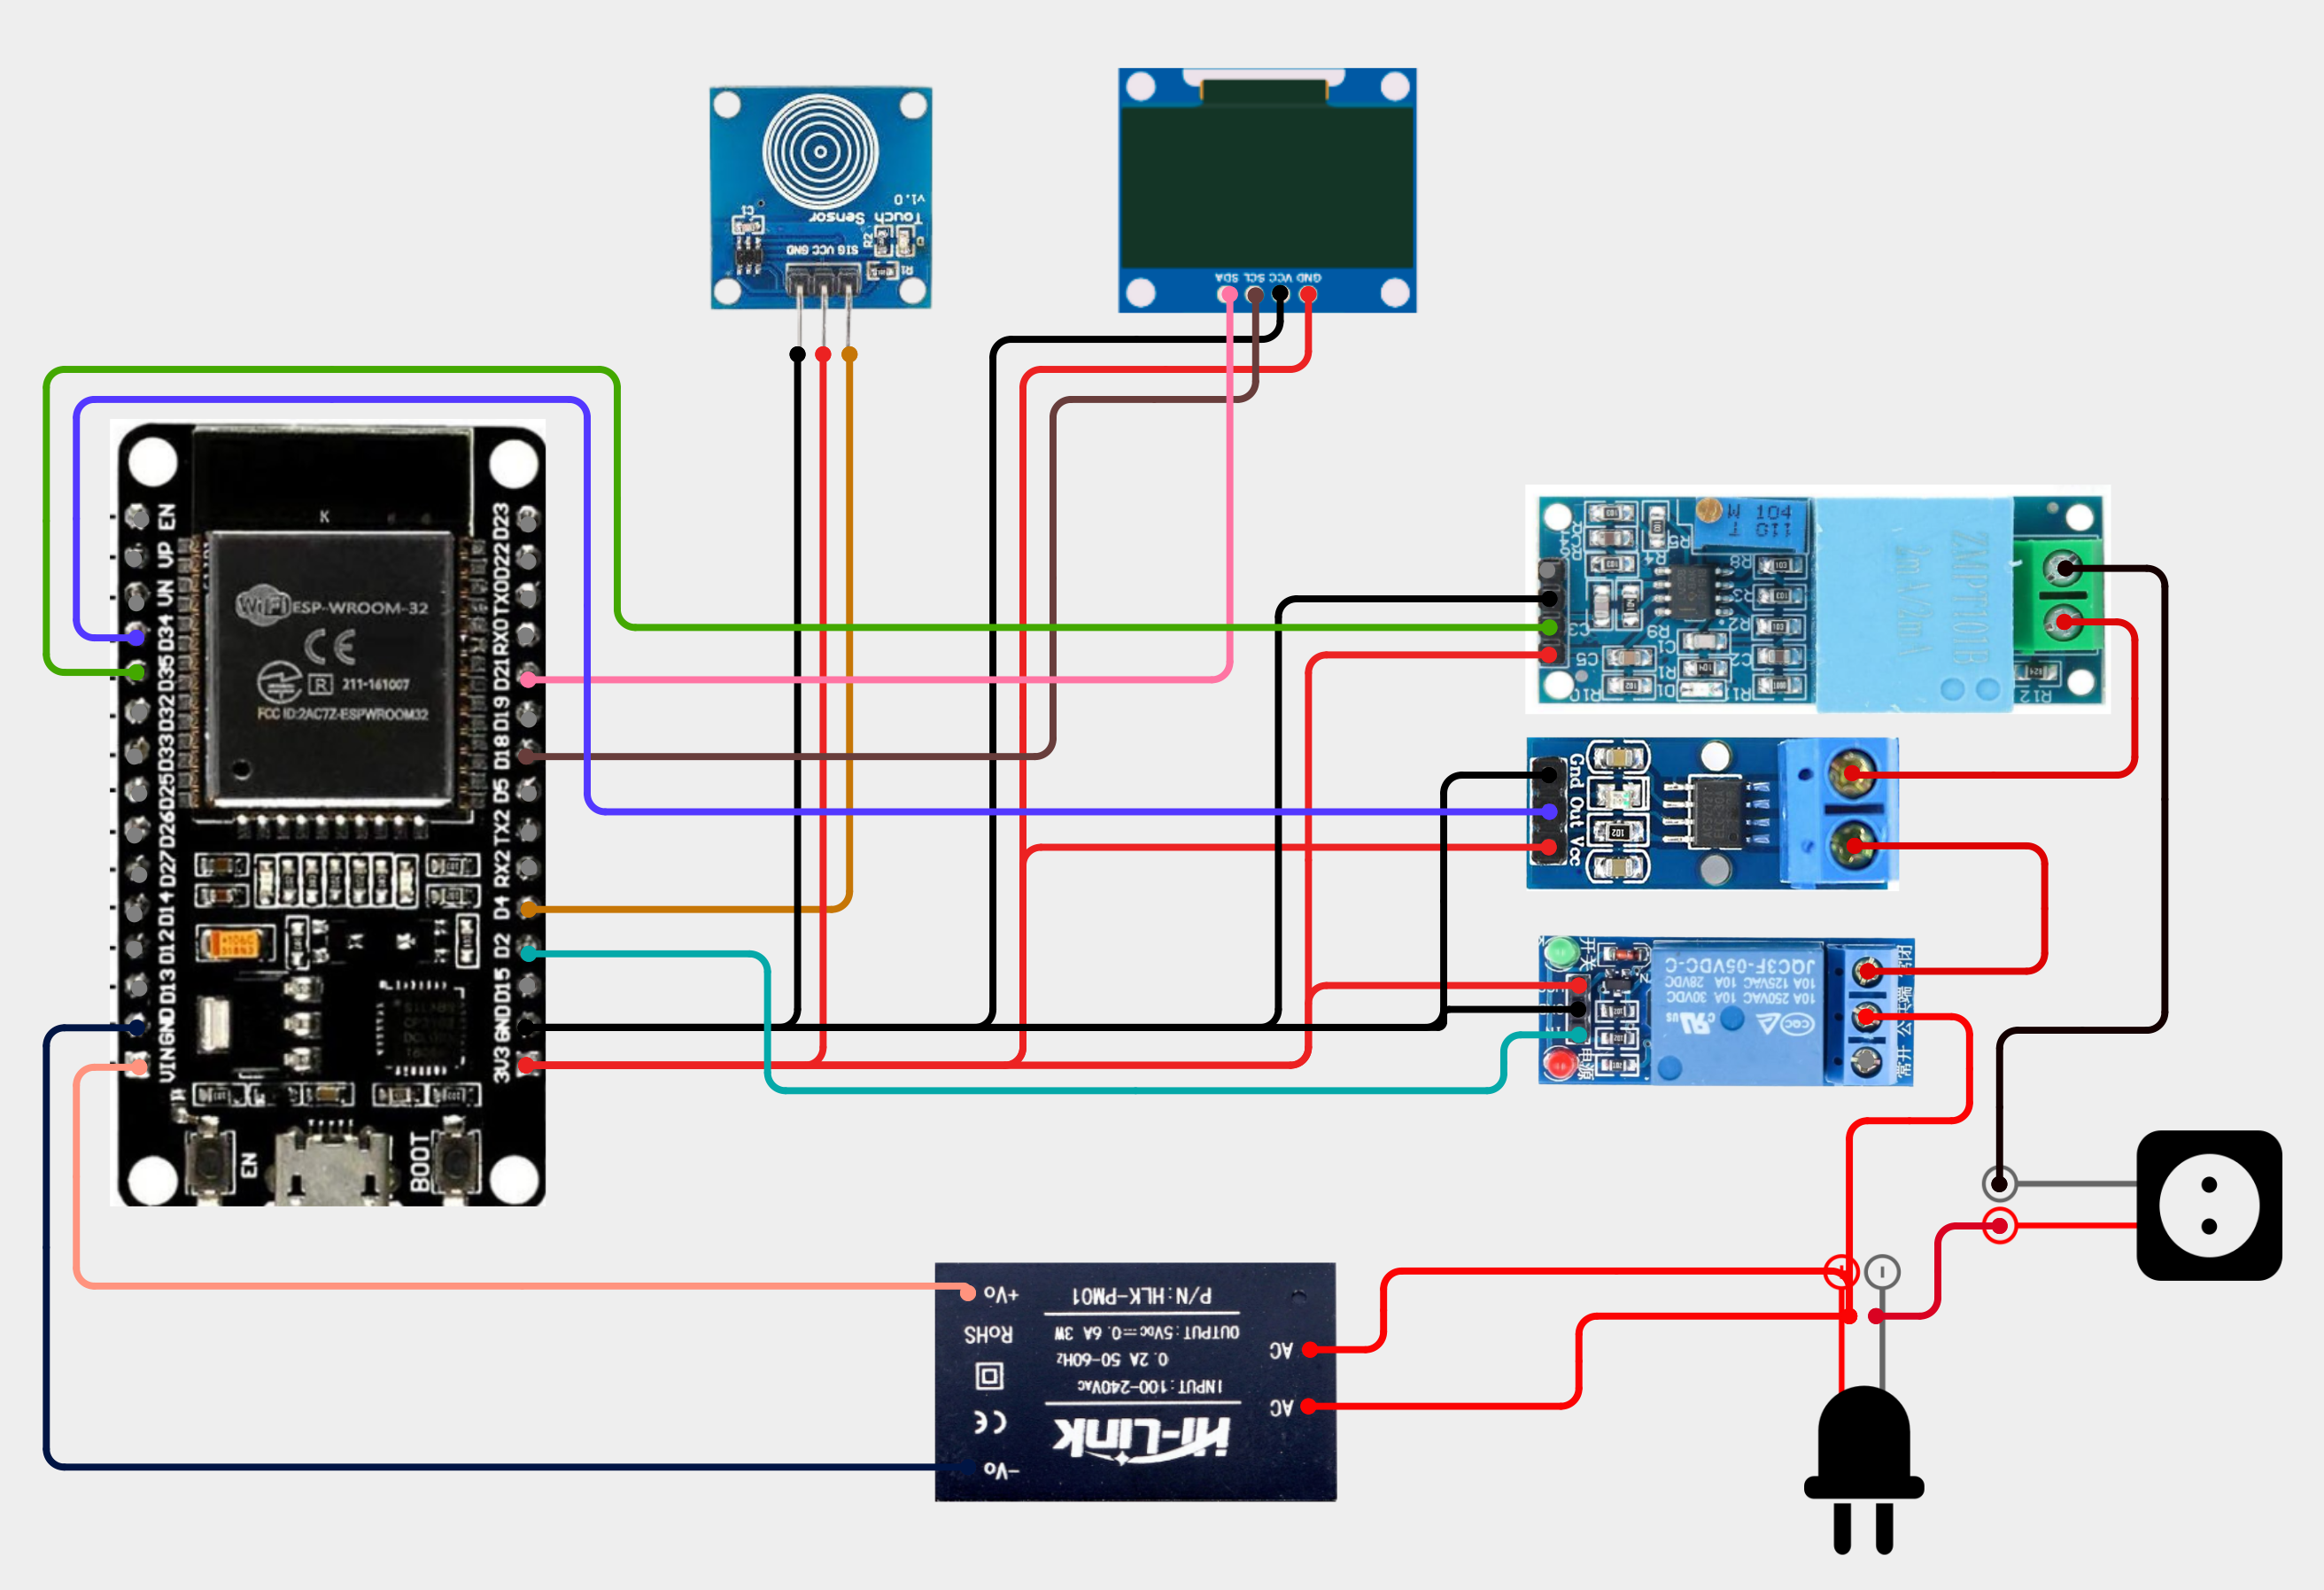
\includegraphics[width=0.95\textwidth]{circuit_image.png}
		\caption{Circuit diagram of the Smart Energy Meter}
		\label{fig:circuit}
	\end{figure}
	
	\subsection{Description of Component}
	
	\begin{table}[H]
		\centering
		\caption{GPIO pin assignments}
		\label{tab:gpio}
		\vspace{6pt}
		\begin{tabular}{|c|l|l|l|}
			\hline
			\textbf{GPIO} & \textbf{Function} & \textbf{Direction} & \textbf{Connected to} \\
			\hline
			35 & Voltage ADC & Input & ZMPT101B output \\
			34 & Current ADC & Input & ACS712 output \\
			18 & I2C SCL & Output & OLED clock \\
			21 & I2C SDA & Bidirectional & OLED data \\
			2 & Relay control & Output & Relay IN (active LOW) \\
			4 & Touch sensor & Input & TTP223 output \\
			\hline
		\end{tabular}
	\end{table}
	
	\begin{enumerate}[]
	\item \textbf{Power supply:} The HLK-PM01 converts 230V AC mains to 5V DC. The ESP32 DevKit V1 has a built-in AMS1117-3.3V regulator that steps down the 5V to 3.3V for the microcontroller and sensors. This eliminates the need for an external 3.3V regulator.
	
	\item \textbf{Voltage measurement:} The ZMPT101B is a miniature voltage transformer with built-in signal conditioning. It outputs a voltage proportional to the input AC voltage, centered at VCC/2 (approximately 1.65V). The ESP32 ADC reads this signal and the firmware computes RMS voltage.
	
	\item \textbf{Current measurement:} The ACS712-20A is a Hall-effect current sensor. Current flowing through the sensor creates a magnetic field that the Hall element converts to a voltage. Sensitivity is 100mV per ampere, with zero-current output at VCC/2.
	
	\item \textbf{Display:} The SSD1306 OLED is a 128x64 pixel monochrome display with I2C interface. It draws approximately 20mA and provides clear visibility in both bright and dim conditions.
	
	\item \textbf{Relay:} The 5V relay module has an optocoupler for isolation. The relay coil is triggered by pulling GPIO 2 LOW. The relay contacts are rated for 10A at 250V AC for resistive loads.
	\end{enumerate}
	
	\subsection{Machine Learning}
	
	The ML pipeline processes historical energy data through four stages. Figure~\ref{fig:ml-stages} shows the data transformation at each stage.
	
	\begin{figure}[H]
		\centering
		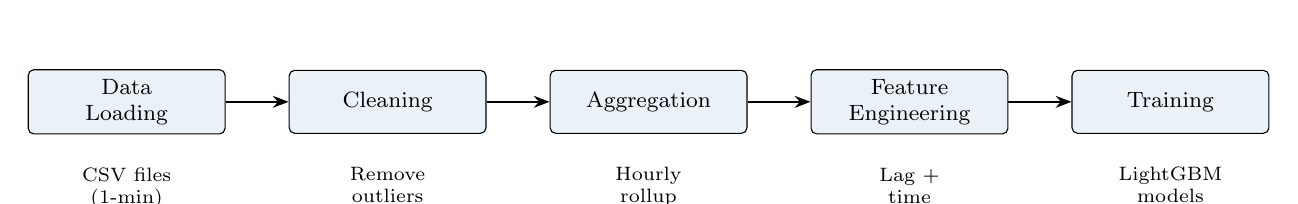
\begin{tikzpicture}[
			node distance=0.8cm,
			stage/.style={rectangle, draw, fill=primaryblue!10, minimum width=2.5cm, minimum height=0.8cm, align=center, font=\footnotesize, rounded corners=2pt},
			arrow/.style={-{Stealth[length=2mm]}, thick}
		]
		\node[stage] (load) {Data\\Loading};
		\node[stage, right=of load] (clean) {Cleaning};
		\node[stage, right=of clean] (agg) {Aggregation};
		\node[stage, right=of agg] (feat) {Feature\\Engineering};
		\node[stage, right=of feat] (train) {Training};
		
		\draw[arrow] (load) -- (clean);
		\draw[arrow] (clean) -- (agg);
		\draw[arrow] (agg) -- (feat);
		\draw[arrow] (feat) -- (train);
		
		% Labels below
		\node[below=0.3cm of load, font=\scriptsize, align=center] {CSV files\\(1-min)};
		\node[below=0.3cm of clean, font=\scriptsize, align=center] {Remove\\outliers};
		\node[below=0.3cm of agg, font=\scriptsize, align=center] {Hourly\\rollup};
		\node[below=0.3cm of feat, font=\scriptsize, align=center] {Lag +\\time};
		\node[below=0.3cm of train, font=\scriptsize, align=center] {LightGBM\\models};
		\end{tikzpicture}
		\caption{ML pipeline stages}
		\label{fig:ml-stages}
	\end{figure}
	
	\begin{itemize}[itemsep=4pt, topsep=6pt]
		\item \textbf{Data loading:} Raw CSV files from the AMPds dataset are loaded and merged with environmental data (temperature, humidity). Column names are normalized for consistency.
		
		\item \textbf{Cleaning:} Rows with quality flags or missing values are dropped. Outliers above the 99.9th percentile are removed. Small gaps (up to 6 readings) are forward-filled.
		
		\item \textbf{Aggregation:} One-minute readings roll up to hourly aggregates. Each hour receives:
		\begin{itemize}[itemsep=1pt, topsep=2pt]
			\item Mean, max, min, and standard deviation of power
			\item Count of on-minutes
			\item Environmental averages (temperature, humidity)
		\end{itemize}
		Hours with less than 300 readings (83\% coverage) are dropped.
		
		\item \textbf{Feature engineering:} Features are extracted to capture usage patterns:
		\begin{itemize}[itemsep=1pt, topsep=2pt]
			\item Time features: hour of day, day of week, month, season
			\item Lag features: power consumption 1, 6, and 24 hours ago
			\item Rolling statistics: 6-hour mean, 24-hour mean
		\end{itemize}
		
		\item \textbf{Training:} An 80/20 time-based split separates training and validation data. LightGBM trains with early stopping based on validation MAE. Models serialize to .pkl files for deployment.
	\end{itemize}
	\newpage
	
	\section{Implementation / Working}
	
	\subsection{Working Flow}
	
	The following sequence diagram (Figure~\ref{fig:sequence}) shows the data flow from sensor reading to dashboard display. Solid arrows indicate the telemetry path; dashed arrows indicate the relay control path.
	
	\begin{figure}[H]
		\centering
		\resizebox{0.95\textwidth}{!}{%
		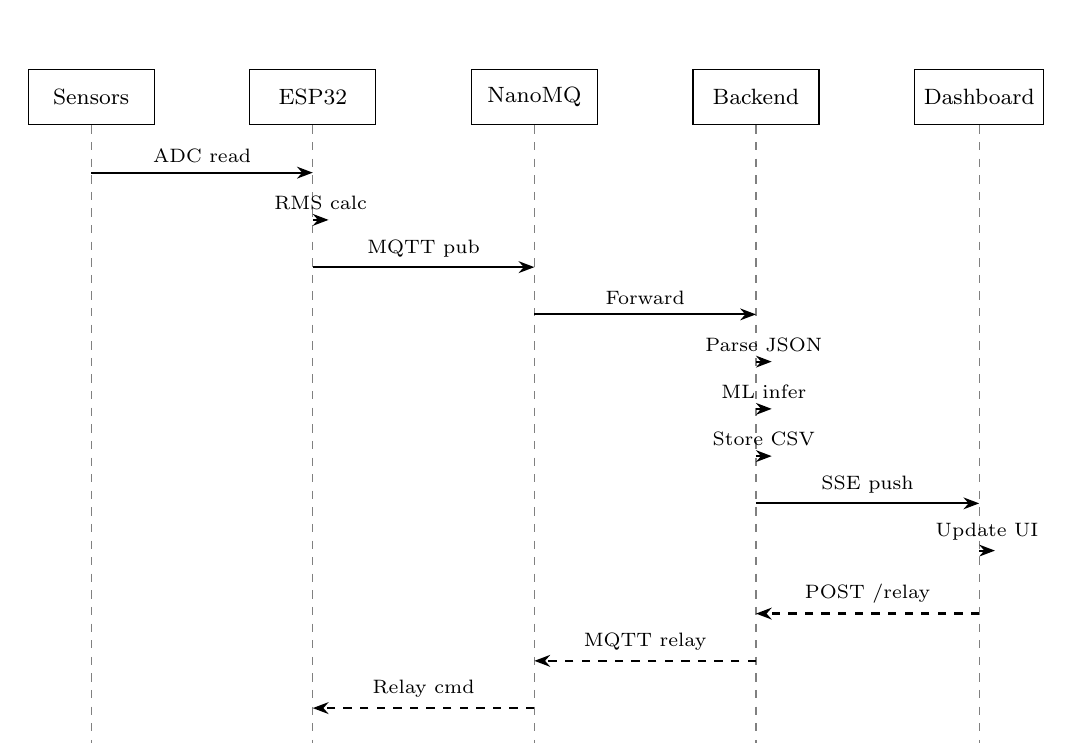
\begin{tikzpicture}[
			node distance=1cm,
			participant/.style={rectangle, draw, minimum height=0.7cm, minimum width=1.6cm, font=\footnotesize},
			arrow/.style={-{Stealth[length=2mm]}, thick},
			msg/.style={font=\scriptsize},
			lifeline/.style={dashed, gray}
		]
		
		% Participants
		\node[participant] (sensors) {Sensors};
		\node[participant, right=1.2cm of sensors] (esp) {ESP32};
		\node[participant, right=1.2cm of esp] (mqtt) {NanoMQ};
		\node[participant, right=1.2cm of mqtt] (backend) {Backend};
		\node[participant, right=1.2cm of backend] (dash) {Dashboard};
		
		% Lifelines
		\draw[lifeline] (sensors.south) -- ++(0,-8);
		\draw[lifeline] (esp.south) -- ++(0,-8);
		\draw[lifeline] (mqtt.south) -- ++(0,-8);
		\draw[lifeline] (backend.south) -- ++(0,-8);
		\draw[lifeline] (dash.south) -- ++(0,-8);
		
		% Messages - Telemetry path
		\draw[arrow] ($(sensors.south)+(0,-0.6)$) -- node[above, msg] {ADC read} ($(esp.south)+(0,-0.6)$);
		\draw[arrow] ($(esp.south)+(0,-1.2)$) -- node[above, msg] {RMS calc} ($(esp.south)+(0.2,-1.2)$);
		\draw[arrow] ($(esp.south)+(0,-1.8)$) -- node[above, msg] {MQTT pub} ($(mqtt.south)+(0,-1.8)$);
		\draw[arrow] ($(mqtt.south)+(0,-2.4)$) -- node[above, msg] {Forward} ($(backend.south)+(0,-2.4)$);
		\draw[arrow] ($(backend.south)+(0,-3.0)$) -- node[above, msg] {Parse JSON} ($(backend.south)+(0.2,-3.0)$);
		\draw[arrow] ($(backend.south)+(0,-3.6)$) -- node[above, msg] {ML infer} ($(backend.south)+(0.2,-3.6)$);
		\draw[arrow] ($(backend.south)+(0,-4.2)$) -- node[above, msg] {Store CSV} ($(backend.south)+(0.2,-4.2)$);
		\draw[arrow] ($(backend.south)+(0,-4.8)$) -- node[above, msg] {SSE push} ($(dash.south)+(0,-4.8)$);
		\draw[arrow] ($(dash.south)+(0,-5.4)$) -- node[above, msg] {Update UI} ($(dash.south)+(0.2,-5.4)$);
		
		% Return path for relay control
		\draw[arrow, dashed] ($(dash.south)+(0,-6.2)$) -- node[above, msg] {POST /relay} ($(backend.south)+(0,-6.2)$);
		\draw[arrow, dashed] ($(backend.south)+(0,-6.8)$) -- node[above, msg] {MQTT relay} ($(mqtt.south)+(0,-6.8)$);
		\draw[arrow, dashed] ($(mqtt.south)+(0,-7.4)$) -- node[above, msg] {Relay cmd} ($(esp.south)+(0,-7.4)$);
		
		\end{tikzpicture}%
		}
		\caption{System sequence diagram}
		\label{fig:sequence}
	\end{figure}
	
	The system operates in a continuous loop consisting of the following steps:
	
	\begin{enumerate}[topsep=6pt, itemsep=5pt]
		\item \textbf{Power on and initialization:} The ESP32 DevKit V1 boots and loads calibration constants from flash memory. It then connects to the WiFi network and establishes an MQTT connection with the backend broker.
		
		\item \textbf{Sensor sampling:} The firmware samples 200 ADC readings from the ZMPT101B voltage sensor and 200 readings from the ACS712 current sensor. This occurs over a 20ms window (one AC cycle at 50Hz).
		
		\item \textbf{RMS calculation:} The firmware computes RMS voltage and RMS current using the formula $V_{RMS} = \sqrt{\frac{1}{n}\sum_{i=1}^{n} v_i^2}$. Power is calculated as $P = V_{RMS} \times I_{RMS}$. Energy accumulates by integrating power over time.
		
		\item \textbf{Display update:} Every second, the OLED display refreshes with the latest readings. Users can cycle through four screens by long-pressing the touch sensor.
		
		\item \textbf{MQTT telemetry:} At the configured interval (default 5 seconds), the ESP32 packages readings into a JSON object and publishes it to the MQTT broker.
		
		\item \textbf{Backend processing:} The Flask server receives the message, parses the JSON, runs ML inference, appends data to CSV storage, and pushes an update via SSE.
		
		\item \textbf{Dashboard display:} The web dashboard receives the SSE event and updates the live power gauge, voltage/current readings, and historical chart.
		
		\item \textbf{Relay control:} Users can toggle the relay from either the local touch button or the web dashboard. Commands flow through MQTT and the relay state is synchronized across all interfaces.
		
		\item \textbf{Continuous operation:} Steps 2--8 repeat continuously while the device is powered on.
	\end{enumerate}
	
	\subsection{Calibration Process}
	
	Before deployment, each unit undergoes calibration to account for sensor variations. The process takes approximately 5 minutes and requires a known load (we used a 600W electric kettle).
	
	\begin{itemize}[]
	\item[Step 1:] \textbf{No-load baseline:} With no appliance connected, the relay closes and the system samples 2000 ADC readings from each sensor. This establishes the DC offset (midpoint) for voltage and current. The noise floor is also recorded.
	
	\item[Step 2:] \textbf{Known-load scaling:} The kettle is plugged in and turned on. Five measurements are averaged, comparing the calculated RMS to the known reference (230V, 600W). This yields the scaling factors that convert raw ADC values to actual volts and amperes.
	
	\item[Step 3:] \textbf{Save and verify:} Constants are saved to \texttt{calibration.json} in flash memory. The display shows measured values for verification against a reference meter.
	\end{itemize}
	
	The calibration output file has the following format:
	
	\begin{lstlisting}[basicstyle=\ttfamily\small, frame=single]
		{
		  "v_midpoint": 2965,
		  "v_scale": 0.2103,
		  "acs_midpoint_v": 2.373,
		  "acs_sensitivity": 0.1075,
		  "v_noise_threshold": 5.78,
		  "i_noise_threshold": 0.107
		}
	\end{lstlisting}
	
	\subsection{Firmware Operation}
	
	The firmware runs a 20ms tick loop handling multiple concurrent tasks:
	
	\begin{itemize}
	\item \textbf{Sensor reading (every 1 second):} Samples 200 points each from voltage and current ADCs over 20ms. Computes RMS by taking the square root of mean of squares. Applies calibration constants. Calculates power ($P = V \times I$) and accumulates energy.
	
	\item \textbf{Display update (every 1 second):} Refreshes the current OLED screen with the latest readings. Cycles through screens on long press of the touch sensor.
	
	\item \textbf{Touch handling (continuous):} Monitors GPIO 4 for touch events. A short tap (50--600ms) toggles the relay. A long press (greater than 600ms) advances to the next display screen.
	
	\item \textbf{Auto-zero compensation:} When the relay turns off, the system waits 300ms for current to settle, then re-measures the ACS712 baseline. This compensates for temperature drift in the Hall-effect sensor.
	
	\item \textbf{MQTT publishing (configurable interval):} Packages voltage, current, power, energy, and relay state into JSON format and publishes to the telemetry topic.
	\end{itemize}
	
	\newpage
	\subsection{Measured Parameters}
	
	Table \ref{tab:params} lists the electrical parameters measured and calculated by the system.
	
	\begin{table}[H]
		\centering
		\caption{Measured electrical parameters}
		\label{tab:params}
		\vspace{6pt}
		\begin{tabular}{|l|l|p{6cm}|}
			\hline
			\textbf{Metric} & \textbf{Formula} & \textbf{Description} \\
			\hline
			RMS Voltage & $\sqrt{\frac{1}{n}\sum v^2}$ & True voltage accounting for AC waveform \\
			RMS Current & $\sqrt{\frac{1}{n}\sum i^2}$ & True current with dynamic zero compensation \\
			Real Power & $V \times I \times PF$ & Actual power consumed (W) \\
			Apparent Power & $V \times I$ & Total power drawn from supply (VA) \\
			Power Factor & $\frac{\text{Real}}{\text{Apparent}}$ & Efficiency metric (0--1) \\
			Energy & $\int P \, dt$ & Cumulative consumption (kWh) \\
			\hline
		\end{tabular}
	\end{table}
	
	\newpage
	
	\section{Result / Output}
	
	This section presents the outputs from each module of the system. The results include hardware implementation photos, web dashboard screenshots, ML model performance metrics, and measurement accuracy tests.
	
	\subsection{Hardware Implementation}
	
	Figure~\ref{fig:device} shows the assembled Smart Energy Meter device. The ESP32 DevKit V1 is mounted on a perfboard along with the sensor modules and relay.
	
	\begin{figure}[H]
		\centering
		\begin{minipage}{0.48\textwidth}
			\centering
			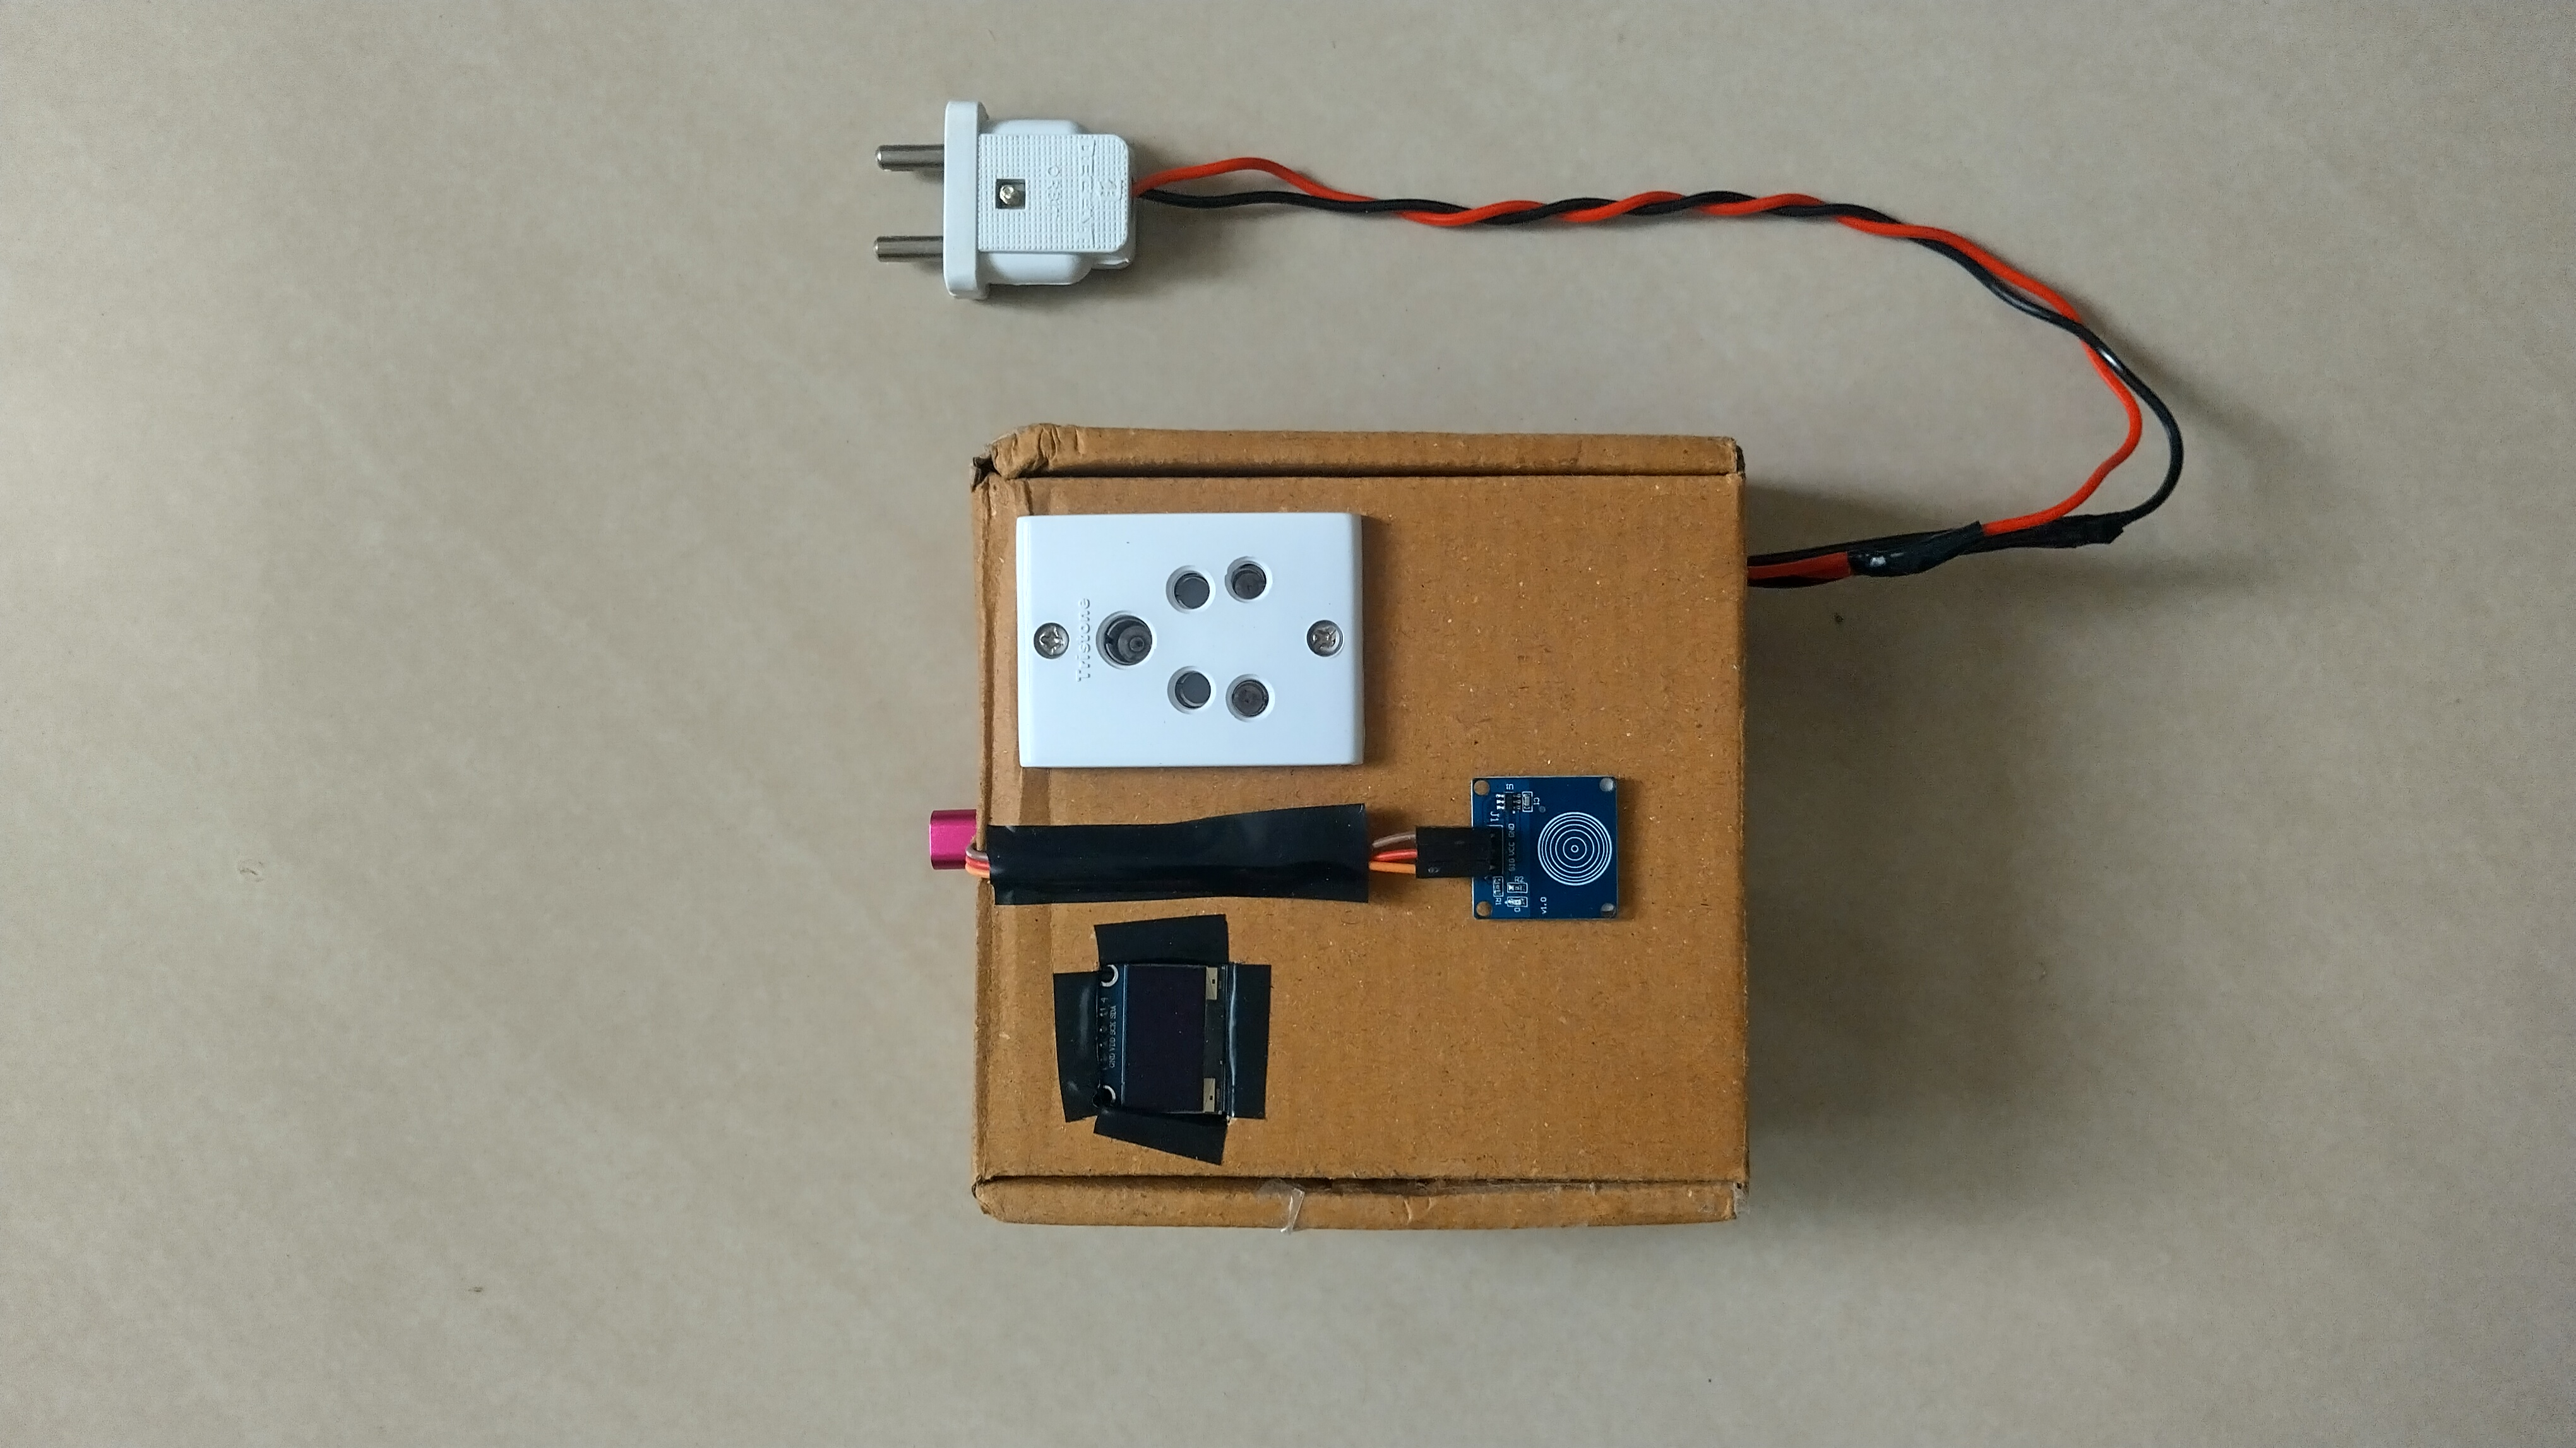
\includegraphics[width=\textwidth]{device.jpg}
			\caption{Assembled device with OLED display showing live readings}
			\label{fig:device}
		\end{minipage}
		\hfill
		\begin{minipage}{0.48\textwidth}
			\centering
			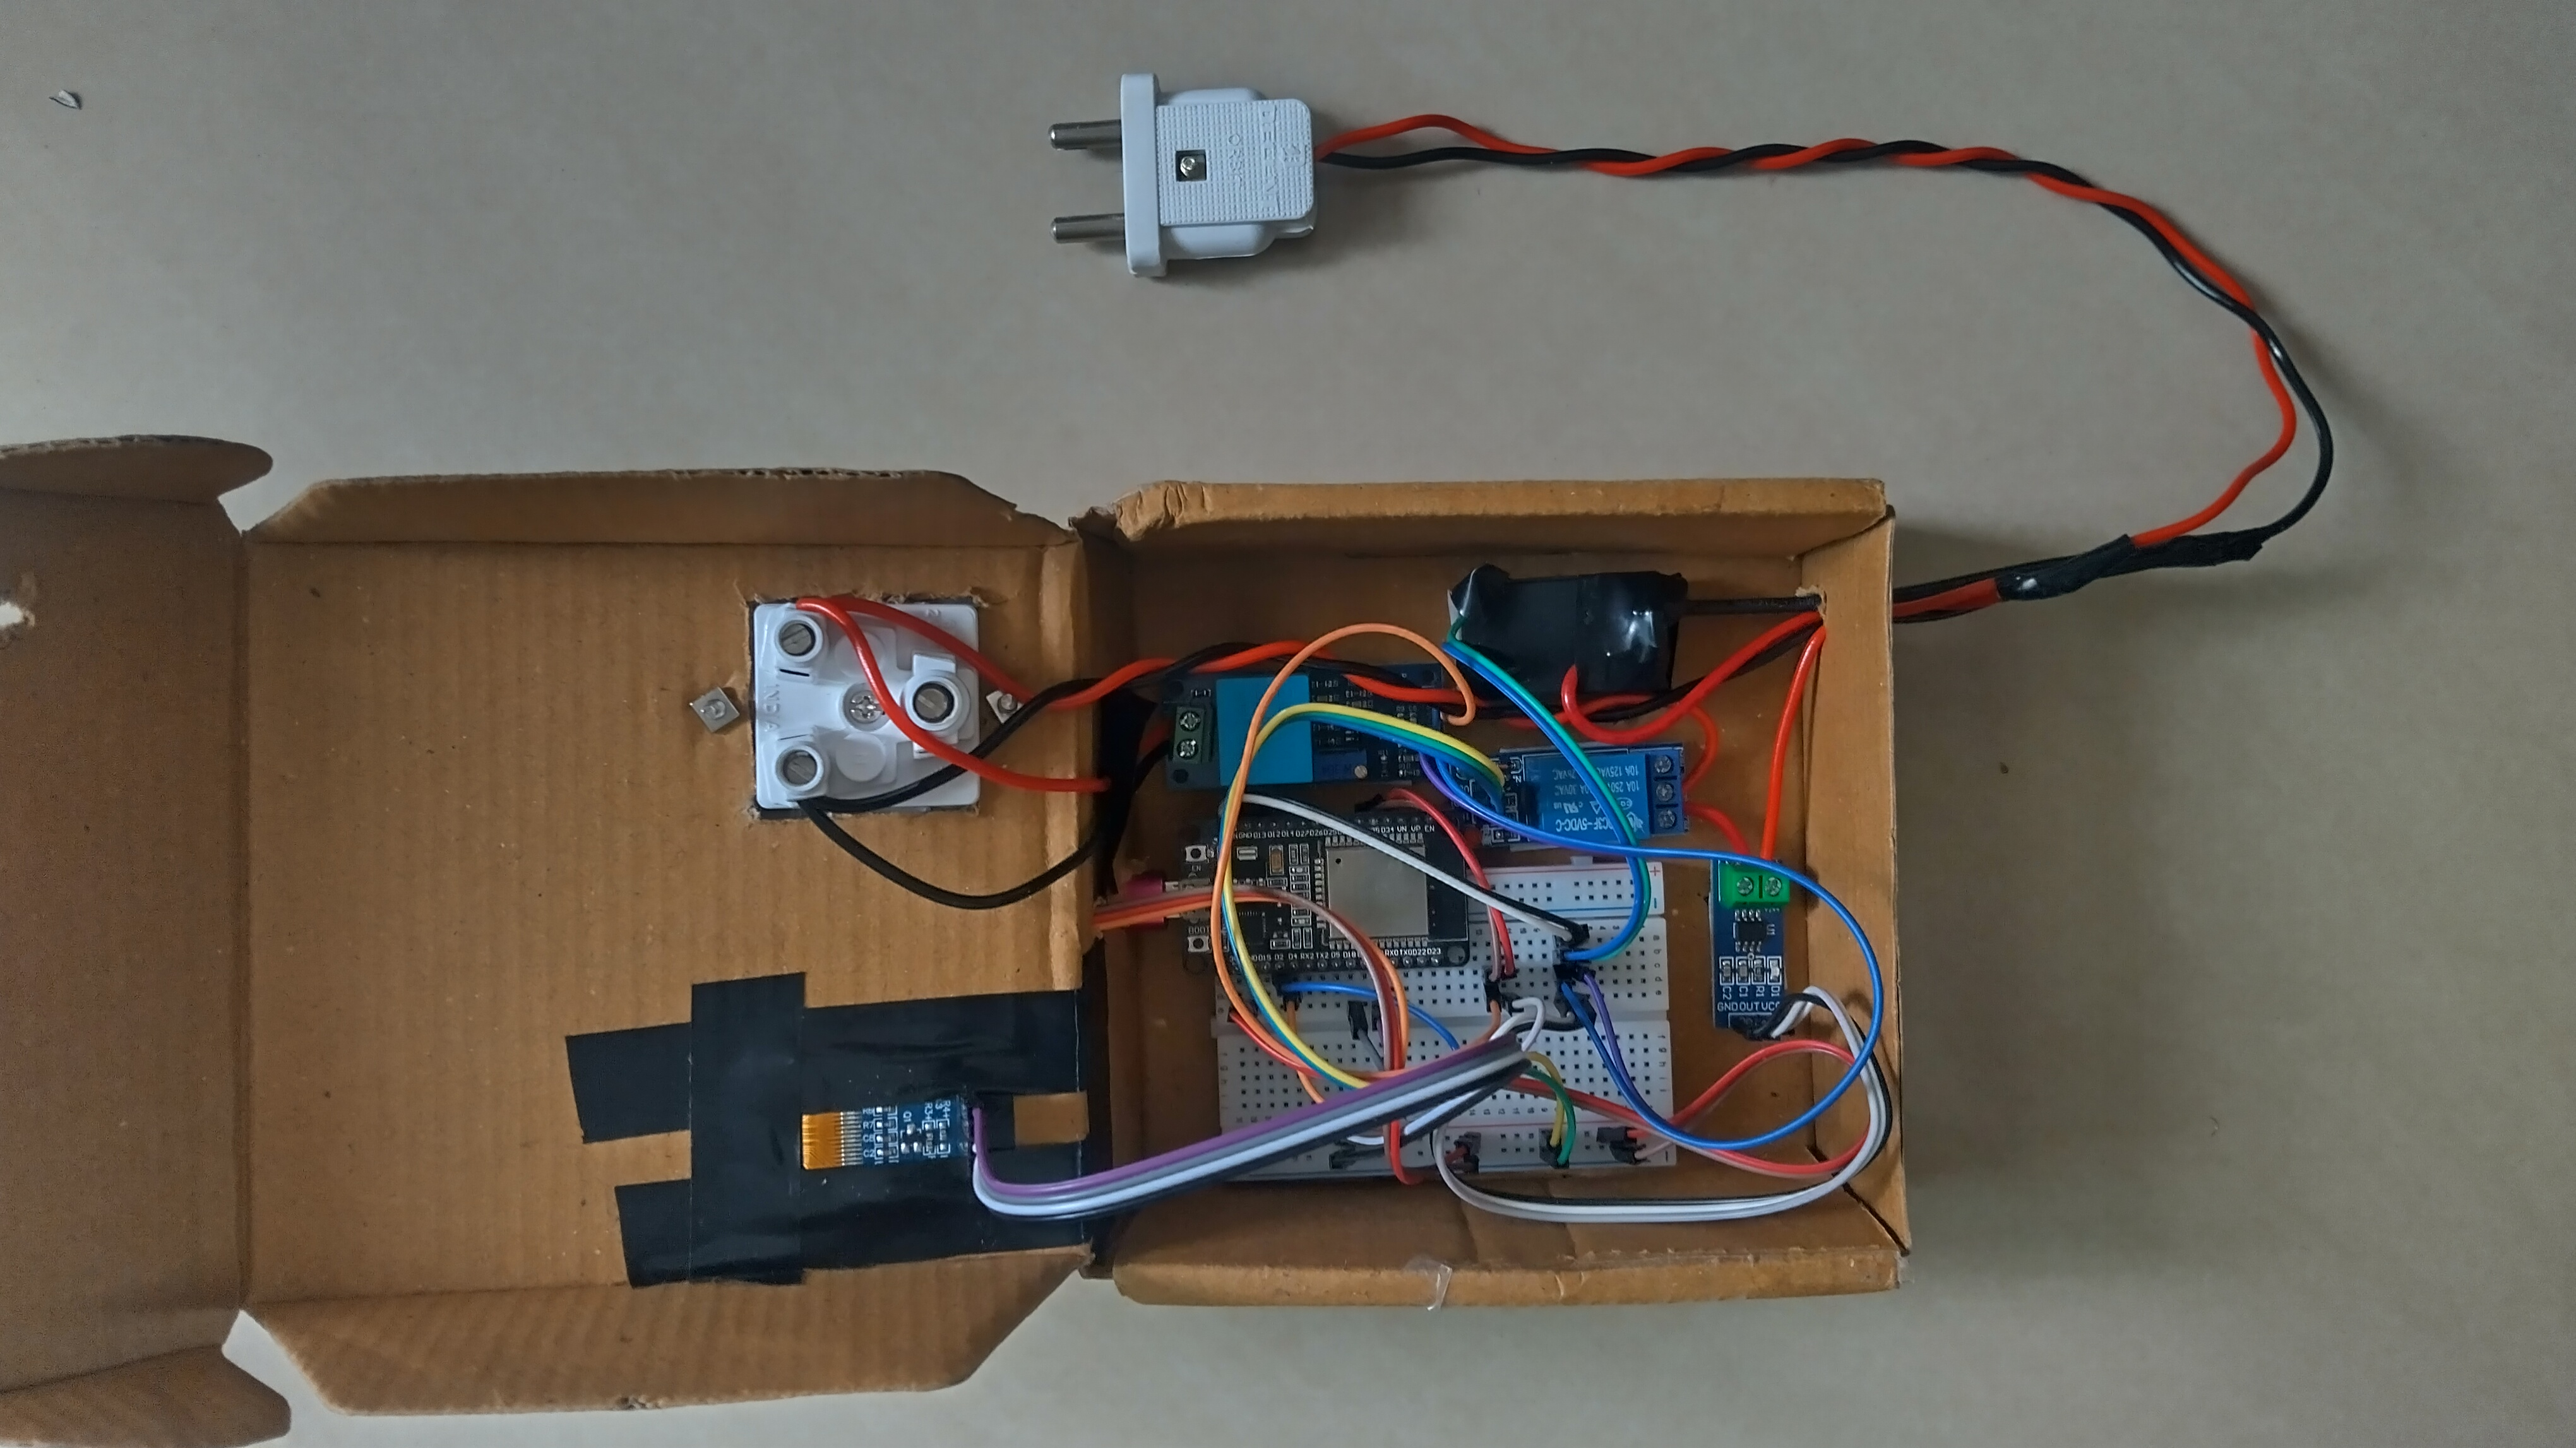
\includegraphics[width=\textwidth]{open-box.jpg}
			\caption{Internal wiring and component layout}
			\label{fig:openbox}
		\end{minipage}
	\end{figure}
	
	\subsection{Testing with Appliances}
	
	We tested the system with an electric kettle (600W rated power). Figure~\ref{fig:kettle-test} shows the kettle connected to the Smart Energy Meter during testing.
	
	\begin{figure}[H]
		\centering
		\begin{minipage}{0.48\textwidth}
			\centering
			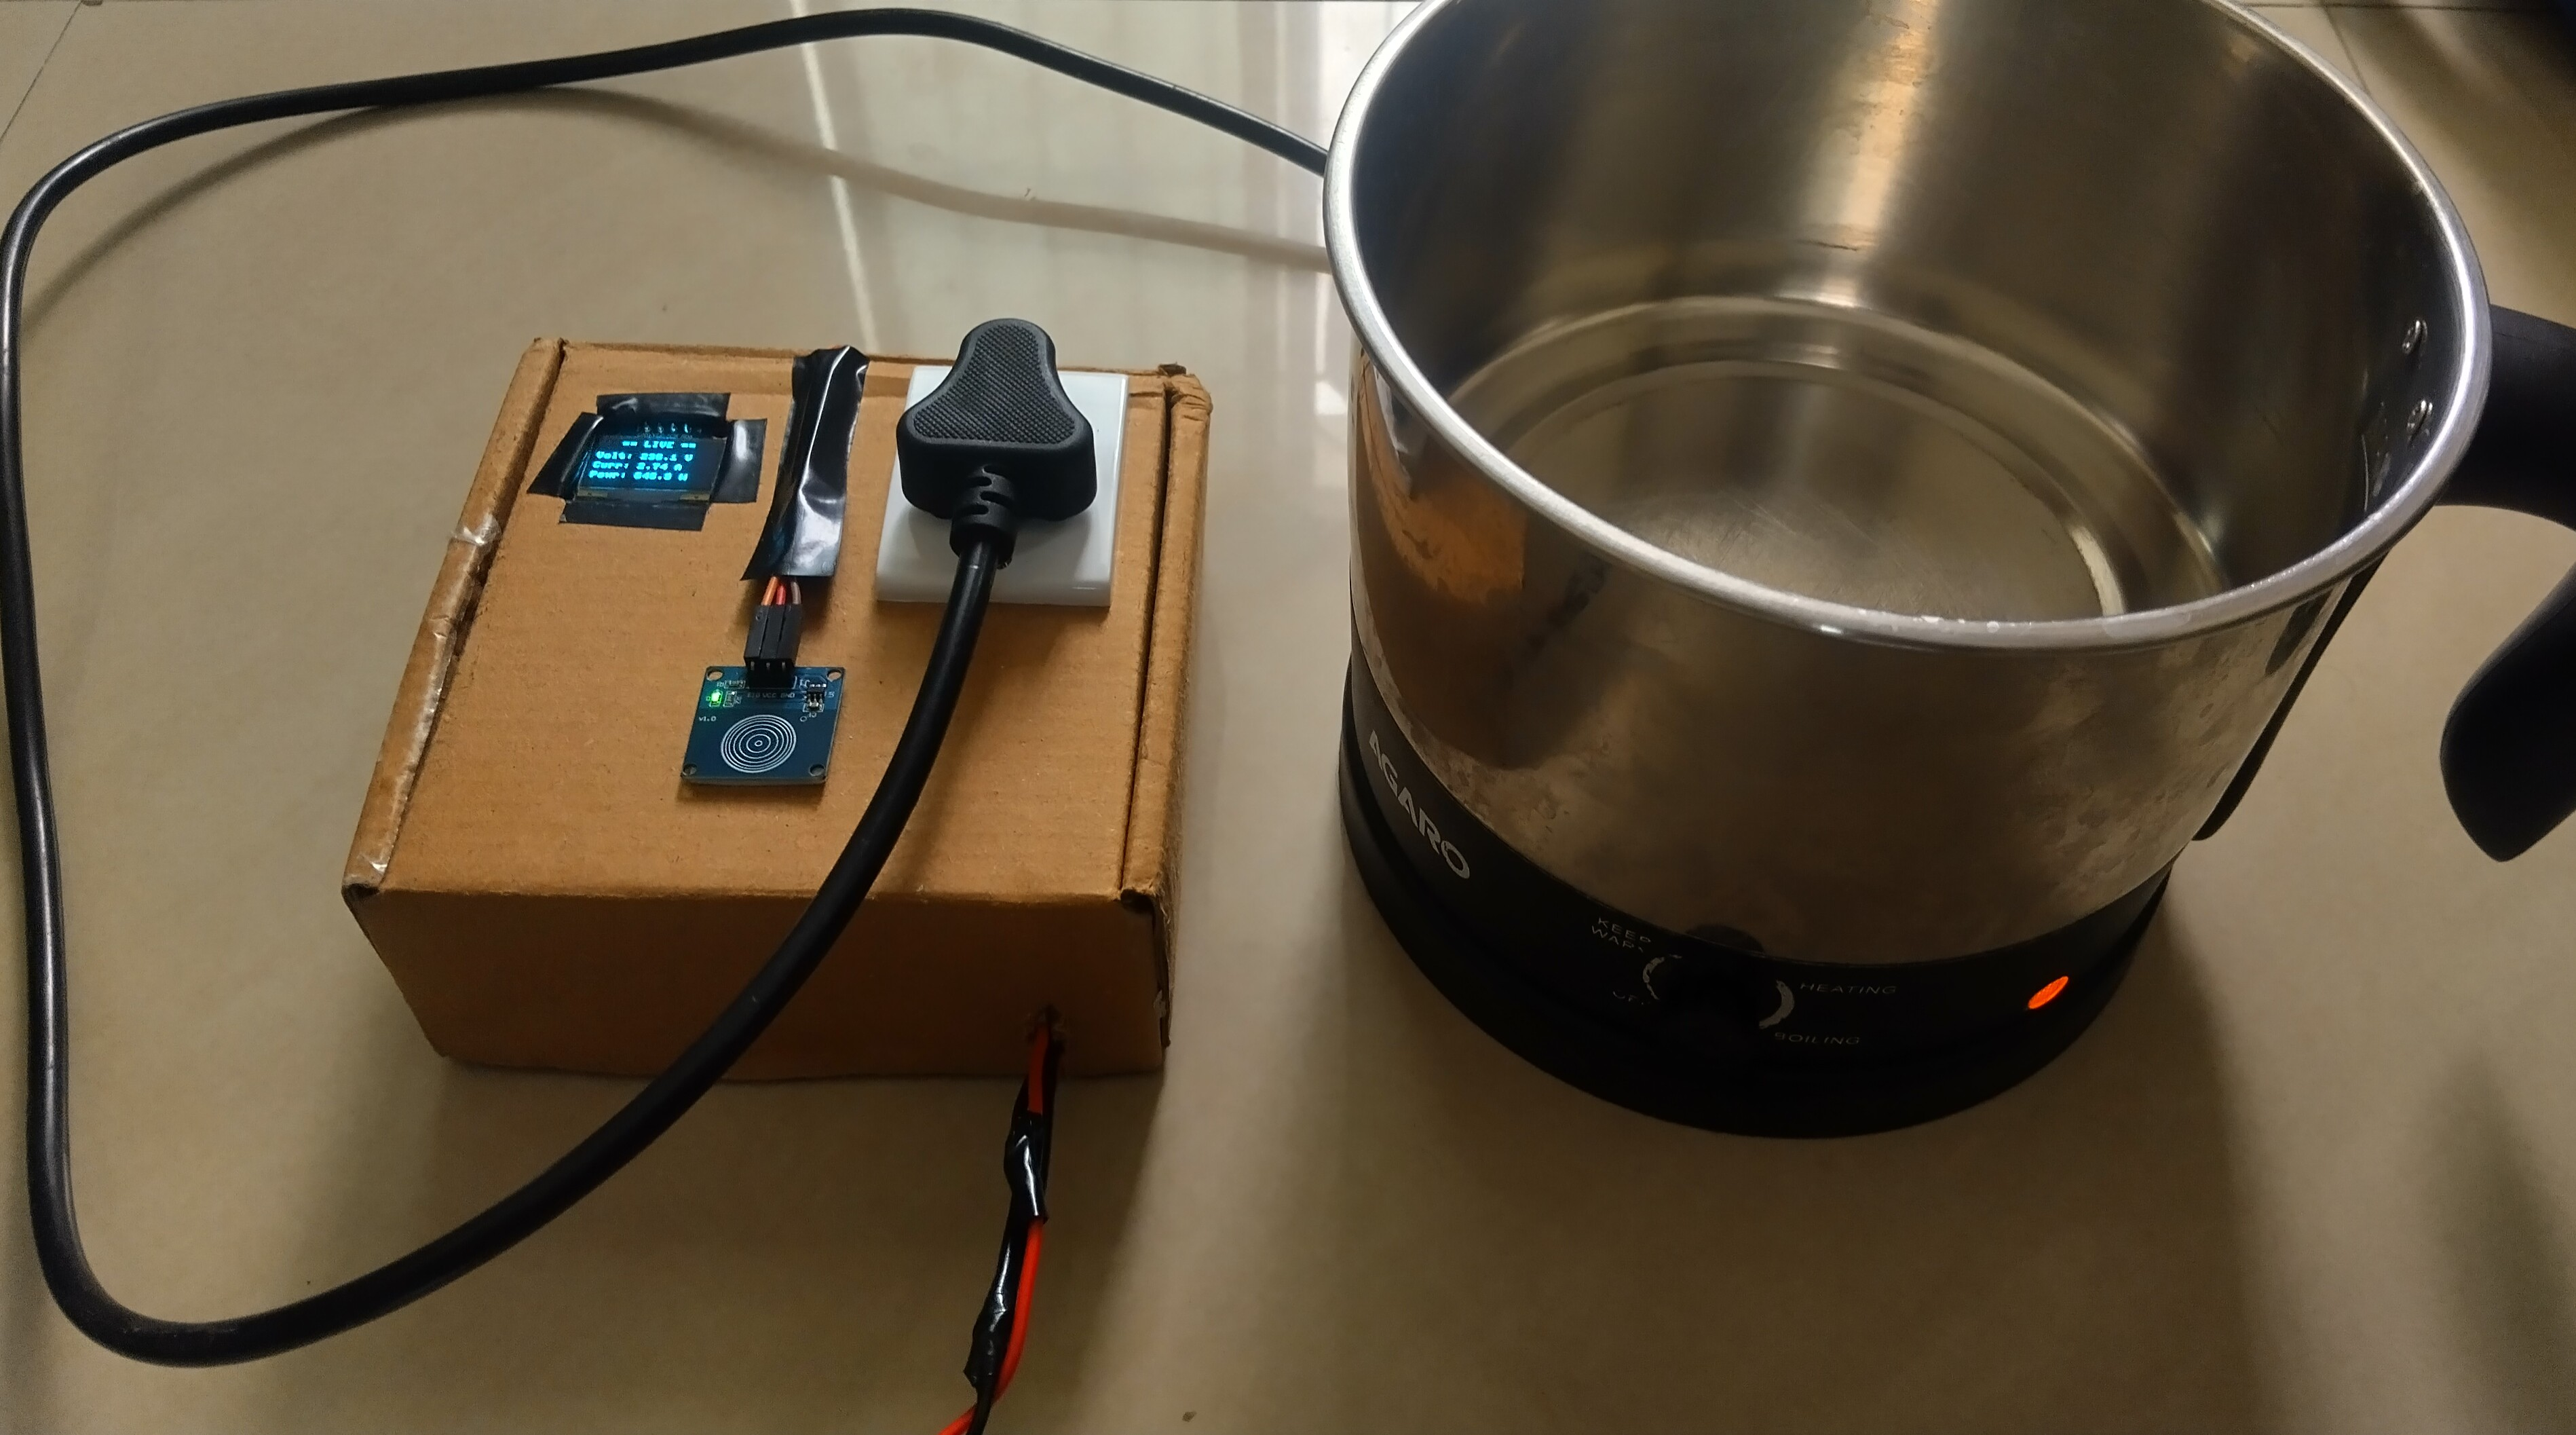
\includegraphics[width=\textwidth]{kettle-test.jpg}
			\caption{Testing setup with electric kettle}
			\label{fig:kettle-test}
		\end{minipage}
		\hfill
		\begin{minipage}{0.48\textwidth}
			\centering
			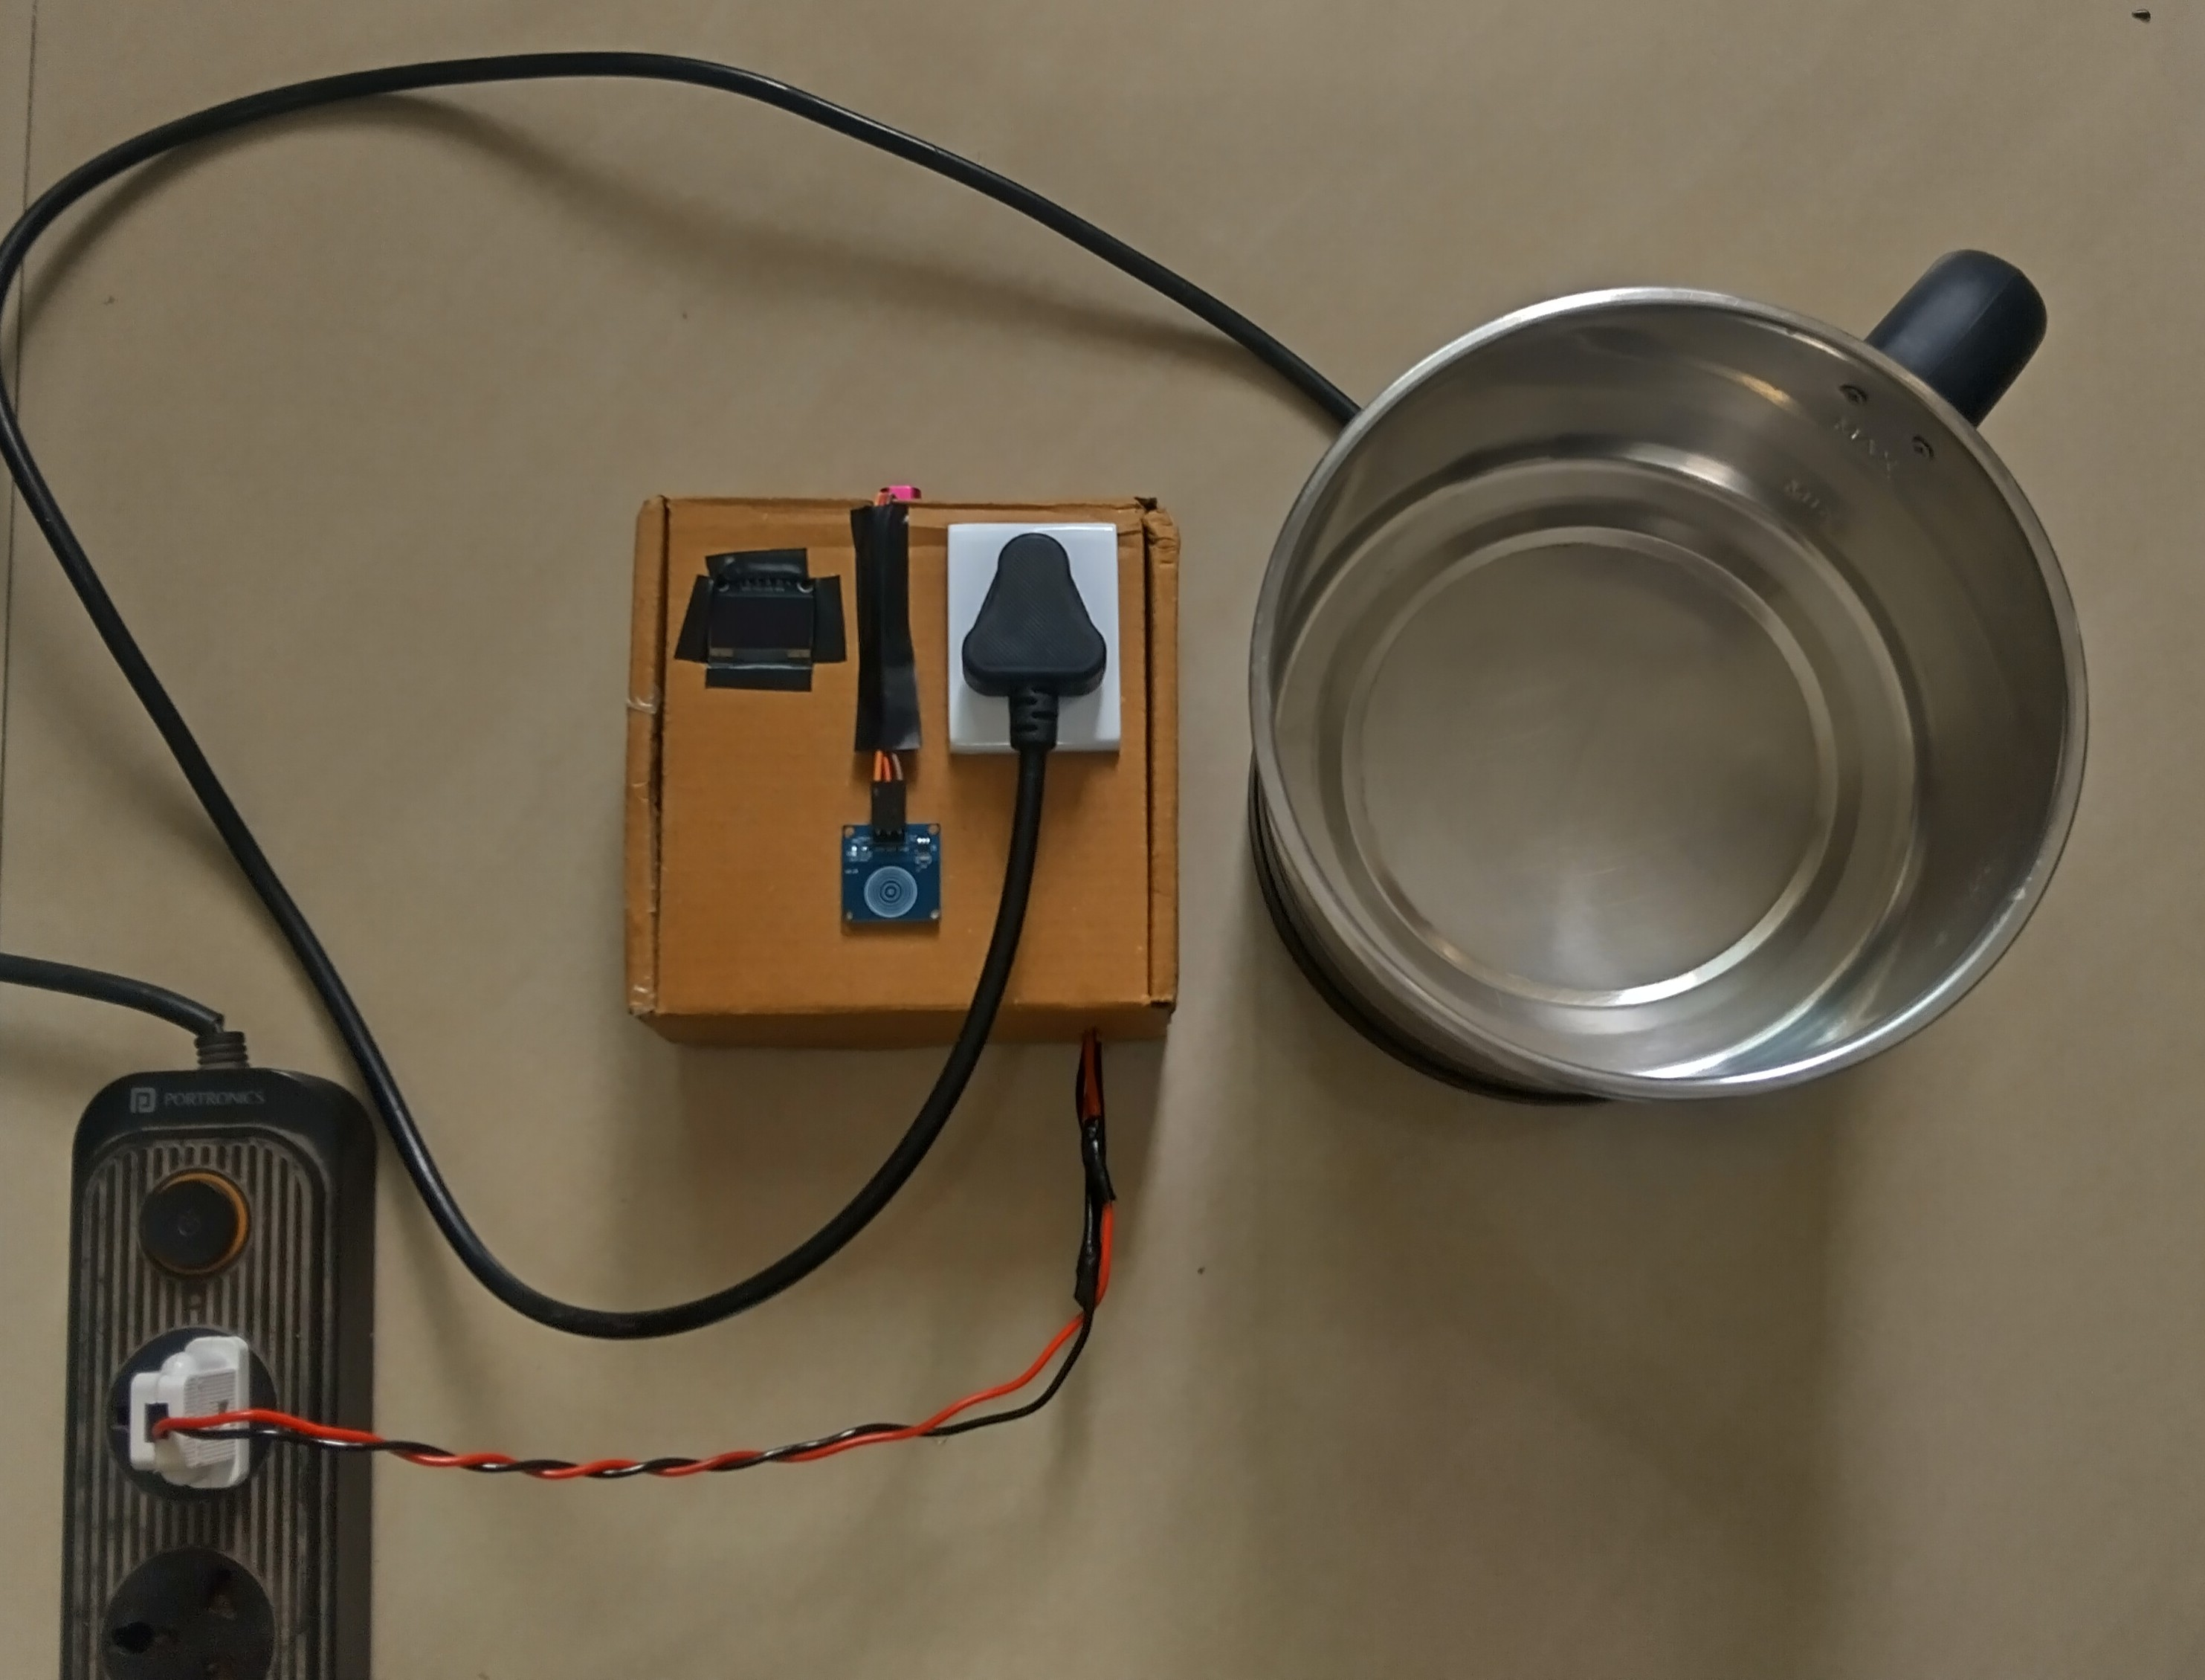
\includegraphics[width=\textwidth]{kettle-tese-2.jpg}
			\caption{Device displaying kettle power consumption}
			\label{fig:kettle-test-2}
		\end{minipage}
	\end{figure}
	
	\subsection{Web Dashboard}
	
	The web dashboard provides remote monitoring and control. Figure~\ref{fig:dashboard} shows the actual dashboard interface.
	
	\begin{figure}[H]
		\centering
		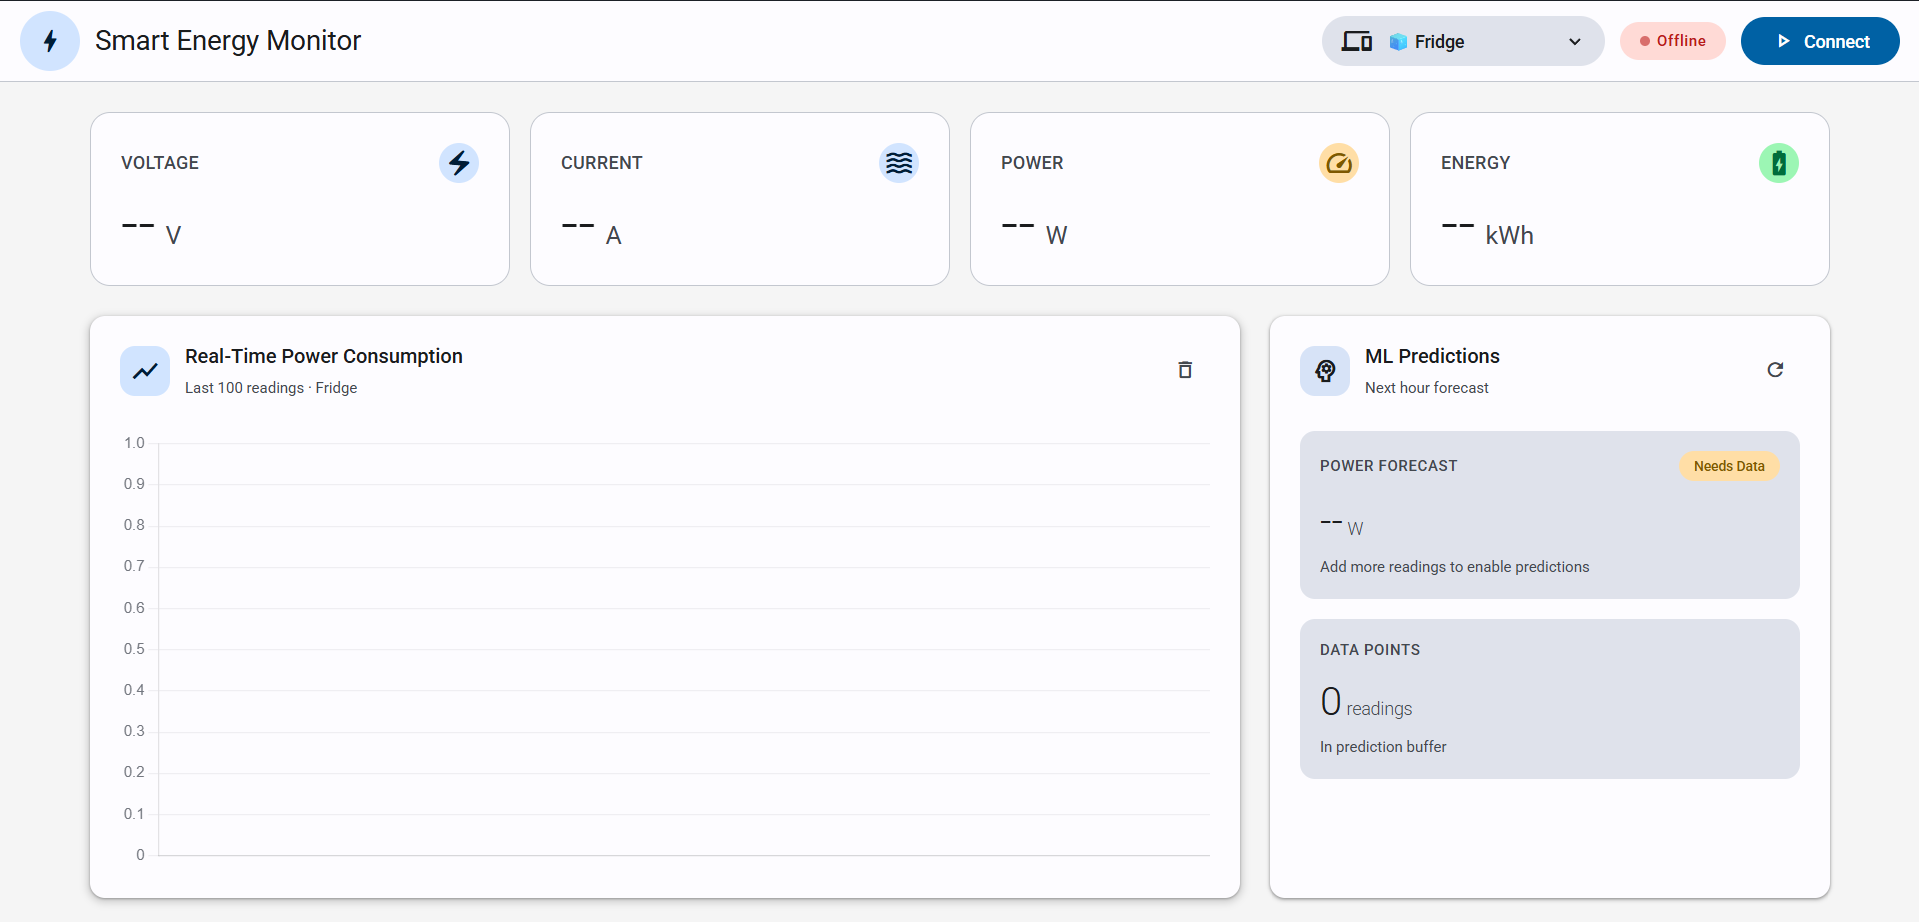
\includegraphics[width=0.85\textwidth]{dashboard.png}
		\caption{Web dashboard showing live power readings and controls}
		\label{fig:dashboard}
	\end{figure}
	
	\begin{figure}[H]
		\centering
		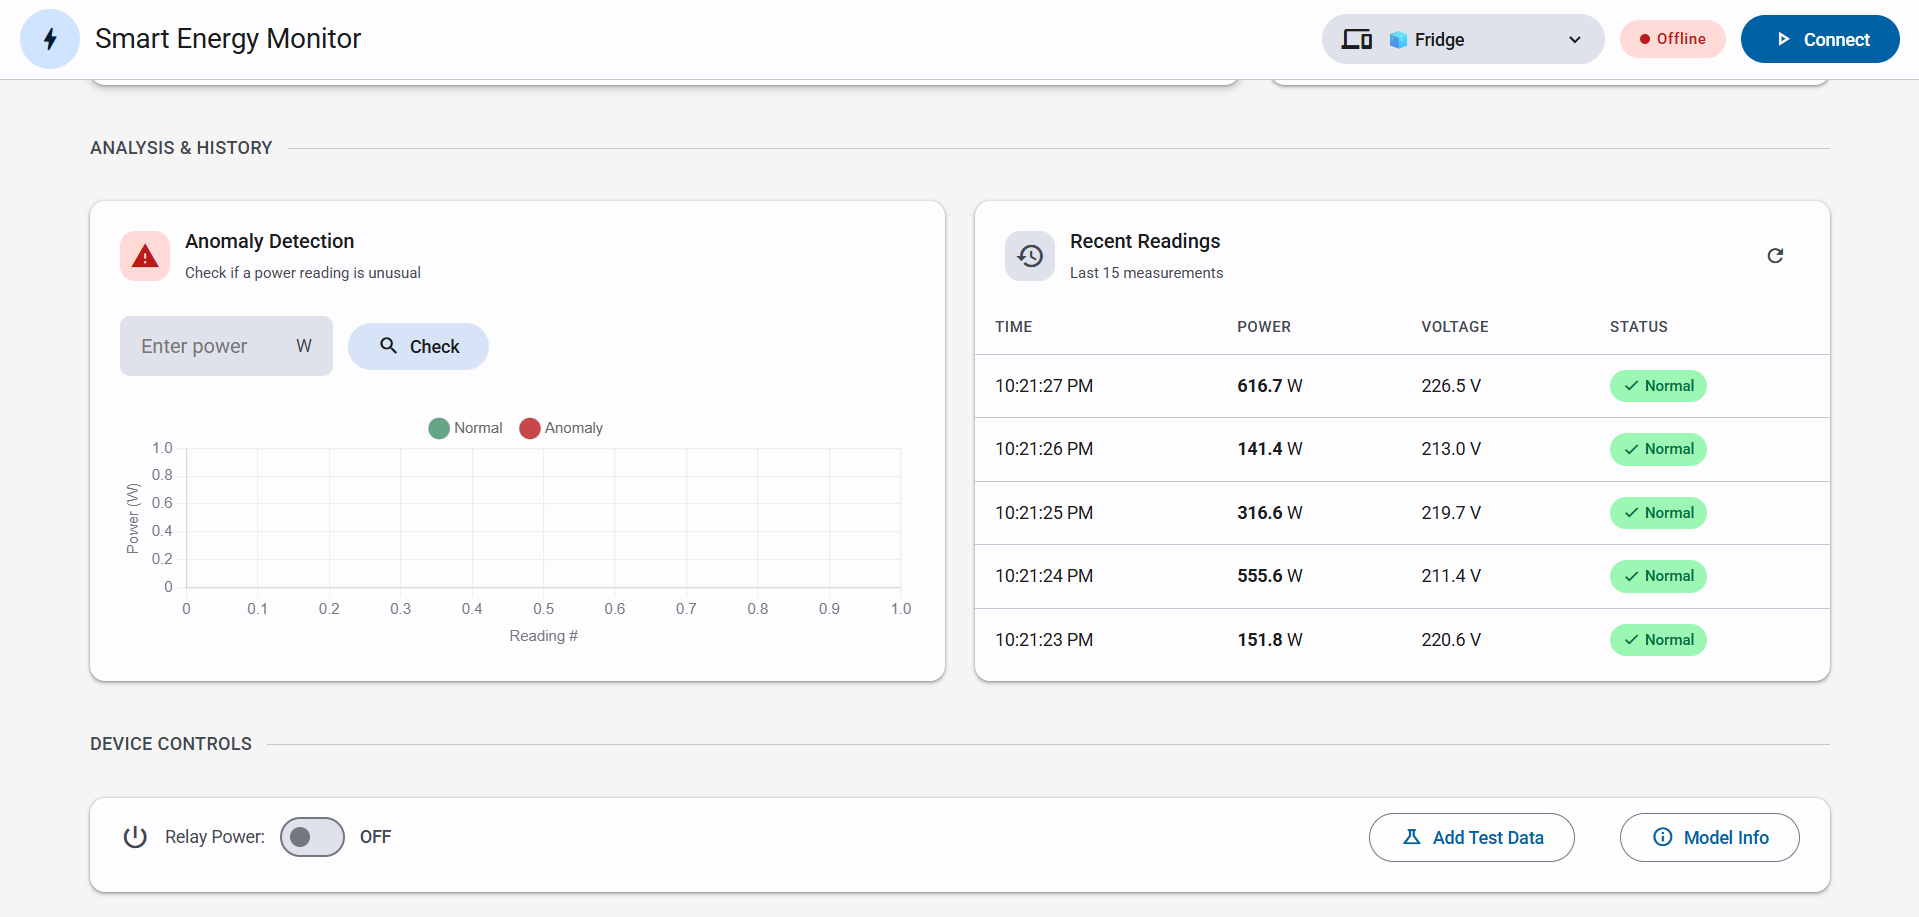
\includegraphics[width=0.85\textwidth]{analysis-history.png}
		\caption{Historical analysis and power consumption graph}
		\label{fig:analysis-history}
	\end{figure}
	
	Dashboard features:
	\begin{itemize}[itemsep=3pt, topsep=4pt]
		\item Live power gauge that updates every second via SSE
		\item Voltage and current readings with units
		\item Historical power chart showing the last 100 readings
		\item Relay toggle button with visual state indicator
		\item Anomaly alert panel (highlighted when ML flags unusual consumption)
		\item Predicted versus actual power comparison
	\end{itemize}
	
	\subsection{OLED Display Screens}
	
	The device has four display screens that cycle when the user long-presses the touch sensor. Table~\ref{tab:oled-screens} describes each screen.
	
	\begin{table}[H]
		\centering
		\caption{OLED display screens}
		\label{tab:oled-screens}
		\vspace{6pt}
		\begin{tabular}{|l|p{8cm}|}
			\hline
			\textbf{Screen} & \textbf{Content} \\
			\hline
			Live & Current voltage (V), current (A), and instantaneous power (W) \\
			\hline
			Energy & Accumulated energy consumption (kWh) and relay state (ON/OFF) \\
			\hline
			Control & Relay state indicator with touch instructions for toggling \\
			\hline
			Debug & Raw calibration values, ADC readings, WiFi status, error count \\
			\hline
		\end{tabular}
	\end{table}
	
	User interaction:
	\begin{itemize}[itemsep=2pt, topsep=4pt]
		\item Short tap (50--600ms): Toggle relay on/off
		\item Long press ($>$600ms): Advance to next screen
	\end{itemize}
	
	\subsection{ML Model Performance}
	
	Table~\ref{tab:ml} shows the performance metrics for the trained ML models. These metrics were measured on the test set (20\% of data, time-ordered split).
	
	\begin{table}[H]
		\centering
		\caption{ML model performance on test set}
		\label{tab:ml}
		\vspace{6pt}
		\begin{tabular}{|l|l|r|p{5cm}|}
			\hline
			\textbf{Model} & \textbf{Metric} & \textbf{Value} & \textbf{Interpretation} \\
			\hline
			Power predictor & MAE & 42.3 W & Average error in power prediction \\
			\hline
			Power predictor & R\textsuperscript{2} & 0.87 & Model explains 87\% of variance \\
			\hline
			On/off classifier & Accuracy & 94\% & Correctly classifies device state \\
			\hline
			Anomaly detector & Precision & 89\% & 89\% of flagged anomalies are real \\
			\hline
		\end{tabular}
	\end{table}
	
	\subsection{Sample Telemetry Data}
	
	A typical telemetry JSON payload transmitted from the ESP32 to the backend:
	
	\begin{lstlisting}[basicstyle=\ttfamily\small, frame=single]
		{
		  "voltage": 228.5,
		  "current": 2.34,
		  "power": 534.7,
		  "energy": 1.234,
		  "relay": true,
		  "timestamp": "2025-04-07T10:30:00"
		}
	\end{lstlisting}
	
	The backend parses this JSON, runs ML inference, stores the data in CSV format, and broadcasts updates to connected dashboards.
	
	\subsection{Measurement Accuracy}
	
	We tested the system against a commercial power meter (calibrated to $\pm$0.5\% accuracy) using two test appliances:
	
	\begin{itemize}[itemsep=3pt, topsep=4pt]
		\item Electric kettle: 600W resistive load
		\item Laptop charger: 65W switching power supply
	\end{itemize}
	
	Table~\ref{tab:accuracy} shows the measurement accuracy after calibration.
	
	\begin{table}[H]
		\centering
		\caption{Measurement accuracy results}
		\label{tab:accuracy}
		\vspace{6pt}
		\begin{tabular}{|l|c|c|}
			\hline
			\textbf{Parameter} & \textbf{Kettle (600W)} & \textbf{Charger (65W)} \\
			\hline
			Voltage error & $\pm$1.5\% & $\pm$1.5\% \\
			\hline
			Current error & $\pm$2\% & $\pm$5\% \\
			\hline
			Power error & $\pm$2.5\% & $\pm$5\% \\
			\hline
		\end{tabular}
	\end{table}
	
	The ACS712 current sensor is the main source of error. At low currents (below 0.5A), the sensor's 100mV/A resolution becomes a limiting factor. For the laptop charger (approximately 0.3A), the current measurement error was higher due to this resolution limitation.
	
	\newpage
	
	\section{Conclusion and Future Work}
	
	\subsection{Conclusion}
	
	This project implemented a per-appliance energy monitoring system using the ESP32 DevKit V1 microcontroller. The system addresses a practical limitation of whole-house electricity meters: they show aggregate consumption without revealing which devices use the most power.
	
	\textbf{What we built:}
	\begin{itemize}[itemsep=3pt, topsep=4pt]
		\item A hardware module using off-the-shelf components (total cost: Rs. 1,500)
		\item Firmware in MicroPython for sensor sampling and MQTT communication
		\item A Flask backend with ML-based anomaly detection
		\item A web dashboard for real-time monitoring and relay control
	\end{itemize}
	
	\textbf{What the ML adds:}
	
	The machine learning component goes beyond simple threshold alerts. The LightGBM power predictor (R\textsuperscript{2} = 0.87) learns usage patterns and can identify when consumption differs from the norm. The Isolation Forest detector catches subtle changes that may indicate equipment degradation. The on/off classifier (94\% accuracy) predicts expected device state.
	
	\textbf{Testing results:}
	
	We tested the system on two appliances: an electric kettle (600W) and a laptop charger (65W). After calibration, the kettle readings matched a reference meter within 2.5\%. The charger readings were within 5\% due to ACS712 sensor limitations at low currents. The relay switches correctly. Dashboard updates arrive in real time via SSE.
	
	\newpage
	\subsection{Future Work}
	
	Several improvements would increase the practical utility of this system:
	
	\begin{itemize}[itemsep=5pt, topsep=6pt]
		\item \textbf{Power factor measurement:} Currently we compute apparent power ($V \times I$). Adding phase angle detection would give true power factor and real power, which matter for motors and inductive loads.
		
		\item \textbf{Three-phase support:} Some residential and most industrial installations use three-phase power. A version with three current sensors could handle these.
		
		\item \textbf{Local storage and sync:} When WiFi drops, readings should buffer in ESP32 flash and sync when connection returns. The current implementation loses data during outages.
		
		\item \textbf{Mobile application:} A native app with push notifications would be more convenient than the web dashboard for receiving alerts.
		
		\item \textbf{Device auto-detection:} The ML classifier could identify appliance types from their power consumption patterns, removing the need for manual labeling.
		
		\item \textbf{Cost integration:} Adding electricity tariff data to display estimated monthly cost per appliance would make consumption data more actionable.
	\end{itemize}
	
	\newpage
	
	\section{References}
	
	\begin{enumerate}[label={[\arabic*]}, leftmargin=*, topsep=6pt, itemsep=6pt]
		\item Espressif Systems, ``ESP32 Technical Reference Manual,'' 2023. \\ Available: \url{https://www.espressif.com/sites/default/files/documentation/esp32_technical_reference_manual_en.pdf}
		
		\item MicroPython Documentation, ``Quick reference for the ESP32,'' 2024. \\ Available: \url{https://docs.micropython.org/en/latest/esp32/quickref.html}
		
		\item G. Ke et al., ``LightGBM: A Highly Efficient Gradient Boosting Decision Tree,'' in Advances in Neural Information Processing Systems, vol. 30, 2017.
		
		\item F. T. Liu, K. M. Ting, and Z.-H. Zhou, ``Isolation Forest,'' in Proc. IEEE Int. Conf. Data Mining (ICDM), 2008, pp. 413--422.
		
		\item S. Makonin, F. Popowich, L. Bartram, B. Gill, and I. V. Bajic, ``AMPds: A Public Dataset for Load Disaggregation and Eco-Feedback Research,'' in Proc. IEEE Electrical Power and Energy Conf., 2013.
		
		\item Allegro MicroSystems, ``ACS712 Fully Integrated, Hall Effect-Based Linear Current Sensor,'' Datasheet, 2020.
		
		\item Hi-Link Electronic, ``HLK-PM01 AC-DC Power Module,'' Datasheet, 2019.
		
		\item Solomon Systech, ``SSD1306 128x64 Dot Matrix OLED/PLED Segment/Common Driver with Controller,'' Datasheet, 2008.
		
		\item OASIS Standard, ``MQTT Version 5.0,'' 2019. \\ Available: \url{https://docs.oasis-open.org/mqtt/mqtt/v5.0/mqtt-v5.0.html}
		
		\item EMQ Technologies, ``NanoMQ: Ultra-lightweight MQTT Broker,'' 2024. \\ Available: \url{https://nanomq.io/}
		
		\item Pallets Projects, ``Flask Web Development,'' 2024. \\ Available: \url{https://flask.palletsprojects.com/}
		
		\item F. Pedregosa et al., ``Scikit-learn: Machine Learning in Python,'' Journal of Machine Learning Research, vol. 12, pp. 2825--2830, 2011.
		
		\item Chart.js Contributors, ``Chart.js Documentation,'' 2024. \\ Available: \url{https://www.chartjs.org/docs/latest/}
		
		\item A. Faruqui, D. Sergici, and A. Sharif, ``The Impact of Informational Feedback on Energy Consumption: A Survey of the Experimental Evidence,'' Energy, vol. 35, no. 4, pp. 1598--1608, 2010.
		
		\item Y. Wang, Q. Chen, T. Hong, and C. Kang, ``Review of Smart Meter Data Analytics: Applications, Methodologies, and Challenges,'' IEEE Trans. Smart Grid, vol. 10, no. 3, pp. 3125--3148, 2019.
	\end{enumerate}
	
\end{document}